\documentclass[11pt]{beamer}





\usepackage{lmodern} 		% Diese beiden packages sorgen für echte 
\usepackage[T1]{fontenc}	% Umlaute.

\usepackage{amssymb, amsmath, color, graphicx, float, setspace, tipa}
\usepackage[utf8]{inputenc} 
\usepackage[english]{babel}
\usepackage[justification=centering]{caption}
\addto\captionsenglish{\renewcommand{\figurename}{}} %Abbildungen nicht bzw. anders beschriften.


%\usepackage[pdfpagelabels,pdfstartview = FitH,bookmarksopen = true,bookmarksnumbered = true,linkcolor = black,plainpages = false,hypertexnames = false,citecolor = black, breaklinks]{hyperref}
%\usepackage{url}
\usepackage{longtable} 		%Seitenübergreifende Tabelle. Vorlage siehe unten
\newtheorem*{bem}{Bemerkung} % Neue Theorem-Umgebung: Bemerkung
\newcommand{\fillframe}{\vskip0pt plus 1filll} 



%-----------------
%BEAMER-SPEZIFISCH
%-----------------

\usetheme{default}
% Verschiedene Varianten von usetheme, usecolortheme und usefonttheme kann man hier ausprobieren: http://deic.uab.es/~iblanes/beamer_gallery/

% \usetheme{
% 	AnnArbor | Antibes | Bergen |
% 	Berkeley | Berlin | Boadilla |
% 	boxes | CambridgeUS | Copenhagen |
% 	Darmstadt | default | Dresden |
% 	Frankfurt | Goettingen |Hannover |
% 	Ilmenau | JuanLesPins | Luebeck |
% 	Madrid | Malmoe | Marburg |
% 	Montpellier | PaloAlto | Pittsburgh |
% 	Rochester | Singapore | Szeged |
% 	Warsaw
% }
%Interessant scheinen: Boadilla, boxes, CambridgeUS, default, (Goettingen), Hannover, Madrid, Montpellier, Pittsburgh, Rochester, Singapore, Szeged, 

\usecolortheme{dove}
% \usecolortheme{
% 	albatross | beaver | beetle |
% 	crane | default | dolphin |
% 	dove | fly | lily | orchid |
% 	rose |seagull | seahorse |
% 	sidebartab | structure |
% 	whale | wolverine
% }

\usefonttheme{structurebold}
% 	default | professionalfonts | serif |
% 	structurebold | structureitalicserif |
% 	structuresmallcapsserif
% }


%\useinnertheme{
% 	circles | default | inmargin |
% 	rectangles | rounded
% } Am besten sein lassen.


% \useoutertheme{
% 	default | infolines | miniframes |
% 	shadow | sidebar | smoothbars |
% 	smoothtree | split | tree
% } Am besten sein lassen.



\setbeamercovered{transparent} %Halbtransparente Overlays (was als nächstes Element auf der Folie gezeigt wird)
\beamertemplatenavigationsymbolsempty % Entfernt Navigationssymbole unten
%\setbeamertemplate{footline}[frame]  % Seitenzahlen
    \setbeamertemplate{footline}{%
    	\raisebox{5pt}{\makebox[\paperwidth]{\hfill\makebox[10pt]{\hyperlink{tableofcontents}{\scriptsize\insertframenumber}}}}}



%---------------------
%--Metainformationen--
%---------------------
\title{Halo and Sub-Halo Finding in Cosmological N-body Simulations}

\author[M. Ivkovic]{
	Mladen Ivkovic
}
\institute[ICS -- UZH]{Institute for Computational Science\\ University of Zurich}

\date[08.12.2017]{08. June 2017}


% \title[Kurzform]{Vortrag zur Berechenbarkeit}
%     Titel des Vortrages
% \subtitle[Kurzform]{Untertitel}
%     Untertitel
% \author[M. Schulz]{Michael Schulz}
%     Autor festlegen
% \institute[IfI -- HU Berlin]{Institut für Informatik\\ Humboldt-Universität zu Berlin}
%     Angabe des Institutes
% \date[26.05.06]{26. Mai 2006}
%     Datum der Präsentation, alternativ kann mittels \date{\today} auch das aktuelle Datum eingetragen werden.
% \logo{\pgfimage[width=2cm,height=2cm]{hulogo}}
%     Die Datei hulogo.pdf (bzw. hulogo.png, hulogo.jpg, hulogo.mps bei Verwendung von pdftex als Backend) als Logo auf allen Folien, hier mithilfe des Paketes pgf.
% \titlegraphic{\includegraphics[width=2cm,height=2cm]{hulogo}}
%     Die Datei hulogo.pdf (bzw. analog wie bei \logo auch entsprechendes Format) als Logo nur auf der Titelseite unter Verwendung des Paketes graphicx.




%-------------------------------
% Neue Befehle
%-------------------------------

\newcommand{\del}{\partial}
%differential d
\newcommand{\de}{\mathrm{d}}

%\newcommand{\ramses}{\textsc{ramses}}
%\newcommand{\phew}{\textsc{phew}}
%\newcommand{\dice}{\textsc{dice}}
\newcommand{\ramses}{\texttt{RAMSES}}
\newcommand{\phew}{\texttt{PHEW}}
\newcommand{\dice}{\texttt{DICE}}

\newcommand{\dt}{\texttt{dice-twobody}}
\newcommand{\ds}{\texttt{dice-levels}}
\newcommand{\cosmo}{\texttt{cosmo}}
\newcommand{\simple}{simple unbinding}
\newcommand{\neigh}{accounting for neighbours}
\newcommand{\iter}{iterative properties determination}
\newcommand{\phewon}{PHEW only}





%===================
% BIBLIOGRAPHY
%===================
\usepackage[backend=bibtex,sorting=nyt,bibencoding=ascii,citestyle=authoryear]{biblatex}
\addbibresource{references.bib}
\usepackage{csquotes} %recommended when using babel and biblatex
%Abbreviations for Bibliography: http://adsabs.harvard.edu/abs_doc/aas_macros.html
\newcommand{\aap}{Astronomy and Astrophysics}
\newcommand{\mnras}{Monthly Notices of the RAS}
\newcommand{\apj}{The Astrophysical Journal}



%------------------------------------------------------------------
%------------------------------------------------------------------
%----------------VORLAGEN------------------------------------------
%----------------VORLAGEN------------------------------------------
%----------------VORLAGEN------------------------------------------
%------------------------------------------------------------------

%Bruch: \frac{}{}
%Kleiner Bruch: \tfrac{}{}
%Gleichungen: \begin{align}
%Delta für partielle Ableitungen: \partial
%Schönes Epsilon: \varepsilon

%Strich: in align-Umgebung, \bar{} oder \overline{}
%Seitenumbruch: \clearpage ; Besser als \newpage, da er floats zwingt, zuerst eingefügt zu werden.
%Zu grosse Zeilenabstände wegen Formelzeichen? -> \vphantom{}, \smash{}
%\newcommand{\BefehlName}[Anzahl_Parameter]{Definitiere neuen Befehl. Den ersten Parameter ruft man mit #1 ab, den zweiten mit #2 etc}

%%FIGUR
%\begin{figure}[htbp]
%\centering
%\includegraphics[width=15cm]{Bild1}%
%\caption{Experimental set-up}%
%\label{1}
%\end{figure}

%%BILD MIT PICINS NEBEN TEXT SETZEN
%\piccaption{Caption\label{label}} 
%\parpic[r]{\fbox{\includegraphics [width=5cm, keepaspectratio]{bild.png}}}
%


%% ZWEI BILDER NEBENEINANDER.
%% Schau, dass die minipages insgesamt nie mehr als 1.0\textwidth haben.
%% Um ein drittes oder viertes Bild einzufügen, ergänze einfach um weitere minipages.
% \begin{figure}[!htb]
% \centering
%   \minipage{0.3\textwidth}
%     \fbox{\includegraphics[height=2.5cm, keepaspectratio]{rsflipflop.png}}%
%     \caption{RS-Flipflop}%
%     \label{fig:rsflipflop}
%   \endminipage\hspace{1cm}   
% %
%   \minipage{0.4\textwidth}
%     \fbox{\includegraphics[height=2.5cm, keepaspectratio]{rsflipfloptakt.png}}%
%     \caption{getaktetes RS-Flipflop}%
%     \label{fig:rsflipfloptakt}
%   \endminipage
% \end{figure}



%% TABELLEN
%% 1) mit tabular
%\begin{center}
%\begin{tabular}[c]{|p{1cm}|p{3cm}|p{3cm}|p{3cm}|}
%\hline
%\multicolumn{2}{|c||}{Stromstärke 0.4A}	&	\multicolumn{2}{c|}{Stromstärke 0.6A}\\
%\hline
%$4T$ in s	&	$T'$		&	$4T$ in s	&	$T'$\\
%\hline
%7.1			&	1.775	&	7.1		& 	1.775\\
%\hline
%7.2			&	1.8		&	7.1		&	1.775\\
%\hline
%7.3			&	1.825	&	7.1		&	1.775\\
%\hline
%\end{tabular}
%\end{center}
%
%% 2) Mit longtable
%\begin{longtable}{p{3.5cm} p{11.5cm}}
%  Blabla & Blabla\\ [2mm] <= Macht 2mm Abstand zwischen Zeilen
%  %
%  Blabla & Blabla \\ [2mm]
%\end{longtable}


%%%%%%%%%%%%%%%%%%%%%%%%%%%%%%%%%%%%%%%%%%%%%%%%%%%%%%%%%%%%%%%%%%%%%%%%%%%%%%%%%%%%%%%%%%%%%%%%%%%%%%%%%%%%%%%%%%%%%%%%%%%%%%%%%%%%%%%%%%%%%%%%%%%%%%%%%%%%%%%%%%%%%%%%%%%%






\begin{document}

% \begin{frame}[Overlay-Aktionen][Optionen]{Titel}{Untertitel}
% 
% Overlay-Aktionen
%     Overlay-Aktionen setzen die Standard-Overlay-Aktionen aller Umgebungen innerhalb des Frames, welche Aktion-Spezifikationen erlauben. Dazu gehören u.a. \item bei Listen und Block-Umgebungen.
% 
%     <+->
%         Sorgt dafür, dass die Elemente stückweise zum Vorschein kommen.
% 
% Optionen
% 
%     allowdisplaybreaks
%         Sorgt durch Aufruf von \allowdisplaybreaks aus AMS-LaTeX für einen Seitenumbruch bei mehrzeiligen Formelumgebungen. Funktioniert nur im Zusammenhang mit der Option allowframebreaks
%     allowframebreaks
%         Passt der Inhalt nicht mehr auf ein Slide, wird er automatisch auf mehrere Slides verteilt. Allerdings ist somit kein Overlay mehr möglich.
%     b,c,t
%         Sorgt dafür, dass der Frame nach unten (b), zentriert (c) oder nach oben (t) ausgerichtet wird.
%     fragile
%         Wird für Quelltextumgebungen, z.B. verbatim, benötigt.
%     label=name
%         Legt einen Namen für ein Frame fest um es später mit \againframe{name} erneut aufrufen zu können.
%     plain
%         Unterdrückt die Anzeige der Überschrift, Fußzeile und Sidebar.
%     squeeze
%         Verkleinert die vertikalen Abstände so weit wie möglich um u.U. mehr auf der Folie unterbringen zu können.
% 


\begin{frame}{}
	\titlepage
\end{frame}

%\begin{frame}{Outline}\label{tableofcontents}
%   \tableofcontents
%\end{frame}







\section{Introduction}


\begin{frame}
	\frametitle{Cosmological N-body Simulations}
	
	\begin{itemize}
		\item N-body simulations are simulations of the motion of particles under the influence of physical forces.
		\item Focus on collisionless dark matter particles: 
		
		\begin{itemize}
			\item   hypothetical type of matter 
			\item 	the only significant interaction between the particles is via gravity
		\end{itemize}
	
	\end{itemize}
	
\end{frame}








\begin{frame}
	\frametitle{Cosmological N-body Simulations}
	
	\begin{itemize}
		\item After some time, the particles will clump together. Such gravitationally bound objects are called \emph{halos}.
		\item Halos themselves may contain self-bound objects, called \emph{subhalos}.
		\item The identification of halos and subhalos is an important tool for problems concerning cosmic structure and its formation.
		\item Codes that perform this task are called \emph{halo-finders}.
	\end{itemize}
	
\end{frame}














\begin{frame}
	\frametitle{Cosmological N-body Simulations}

	\begin{columns}
		\column{.25\textwidth}
			The results of a cosmological simulation of $128^3$ dark
			matter particles at redshift $z = 0$ with $H_0 = 70.4$ and density parameters $\Omega_m = 0.272$ and $\Omega_\Lambda= 0.728$.
			The box length corresponds to 88.8 Mpc.
			\vfill
		\column{.75\textwidth}
			\begin{figure}
				\centering
				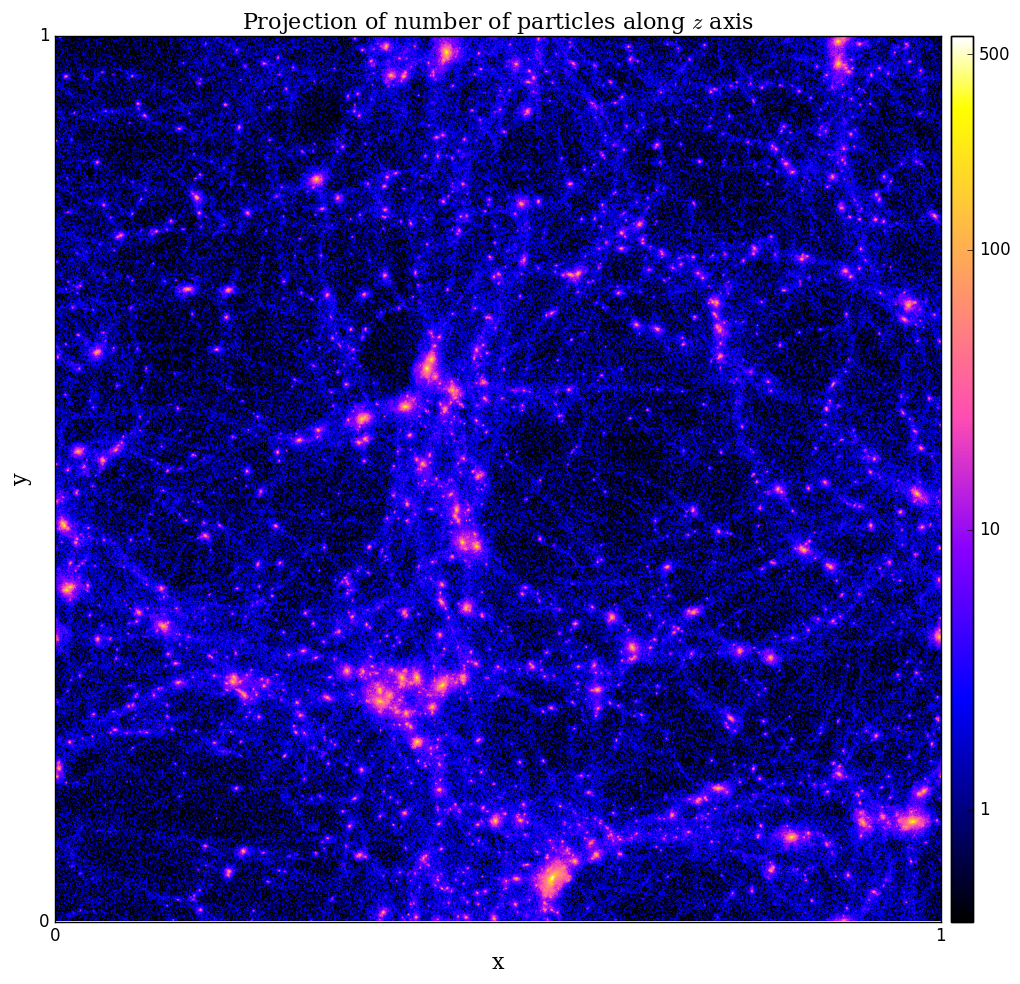
\includegraphics[width=8.2cm]{../report/images/cosmo/cos-part2map-npart.png}
		%		\caption{
		%		}
			\end{figure}
		\vfill
	\end{columns}

\end{frame}










\begin{frame}
	\frametitle{Unbinding Particles}


	\begin{itemize}
		\item By convention, it is customary to treat all particles assigned to a halo as bound to it, even though from a strict energetic perspective they may not be.
		\item For subhalos, on the other hand, it is vital to identify and remove unbound particles:
		\begin{itemize}
			\item Subhalos are located within a host halo and therefore expected to be contaminated by the host's particles
			\item Usually subhalos contain far less particles than their hosts, so assigning particles to it without an unbinding procedure can influence its physical properties significantly.
		\end{itemize}
		\item ``Removing a particle'' means here to assign it to the parent structure. This applies recursively to any level of substructure within substructure.
	\end{itemize}


\end{frame}







\begin{frame}
	\frametitle{Goals of this thesis}


	\begin{itemize}
		\item \ramses\ \parencite{ramses} is a N-body and hydrodynamical code that %
		contains a clump finding algorithm, \phew\ \parencite{PHEW}.
		%makes use of the adaptive mesh refinement technique: The entire computational domain is covered by cells, and smaller and smaller cells are introduced where necessary to achieve the desired accuracy.
%		\item \phew\ \parencite{PHEW} is a clump finding algorithm that can identify halos on-the-fly within the framework of \ramses.
		
		\item Both \phew\ and \ramses\ are fully parallel and make use of the MPI library. \phew\ works on-the-fly.
		
		\item The goal of this thesis is to implement a particle unbinding algorithm to work with \phew\ that is also fully parallel and works on-the-fly.
	\end{itemize}



\end{frame}











\section{PHEW}
\begin{frame}
	\frametitle{PHEW}
	
%	\begin{columns}
%		\column{.6\textwidth}
			\begin{itemize}
				\item \phew\ groups cells together by separating the mass density field along minima, thus dividing the density field into patches.
				
%				\item The density field is obtained with the deposition of the particle’s mass on the mesh through ``Cloud in Cell'' interpolation.
				
				\item The algorithm can	be divided in four main steps:
				
				\begin{itemize}
					\item segmentation
					\item connectivity establishment
					\item noise removal and
					\item substructure merging
				\end{itemize}
			\end{itemize}
%		\column{.4\textwidth}
%			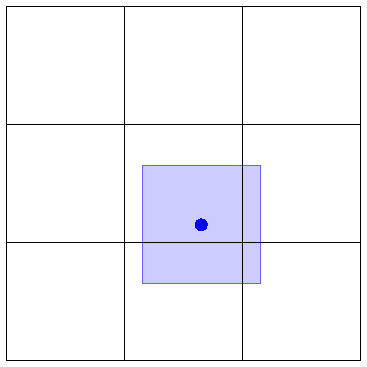
\includegraphics[width = \textwidth, keepaspectratio]{images/tikz/CIC.pdf}
%	\end{columns}
	  
\end{frame}


%\begin{frame}
%	\frametitle{Segmentation}
%	\begin{itemize}
%		\item First, all overdense cells (``test cells'') are identified. If a cell does not have a denser neighbour cell, it is marked as a local density peak and assigned a peak label.
%		
%		\item Then each test cell copies the peak label of its densest neighbour. This way, each cell is assigned
%		to the peak “closest” to it by following the path of rising density.
%		
%		\item All test cells assigned to a particular peak form a peak patch. The separating surface between peak
%		patches will be cell borders which contain local density minima.
%	\end{itemize}
%\end{frame}
%
%\begin{frame}
%	\frametitle{Connectivity Establishment}
%	
%	\begin{itemize}
%		\item For each peak patch, all neighbouring peak patches are identified.
%		The maximal surface density between two particular peak patches is considered as the “saddle” between these two.
%		
%		\item For each peak, out of all the saddles of all the neighbouring peak patches, the one with the highest density is called the “key saddle” and the neighbour it connects to is referred to as the “key neighbour”.
%	\end{itemize}
%	
%\end{frame}
%
%\begin{frame}
%	\frametitle{Noise Removal}
%	\begin{itemize}
%		\item Each peak patch is assigned a value representing the contrast to the background
%		called “relevance”. A peak patch’s relevance is defined as the ratio of the peak’s density to the density of its key saddle. 
%		
%		\item A peak patch is considered noise if the its relevance is lower than a user-defined relevance
%		threshold. 
%		
%		\item An irrelevant peak patch is then merged into its key neighbour or discarded if it has no neighbours.
%		
%		\item Once the noise removal step is completed, the remaining structure consists only of peak patches
%		which satisfy the relevance condition and is referred to as “level 0 clumps”. These clumps represent the structure on the lowest scale.
%	\end{itemize}
%\end{frame}
%
%\begin{frame}
%	\frametitle{Substructure Merging}
%	\begin{itemize}
%		\item The identified level 0 clumps can be merged further into composite clumps.
%		
%		\item All peak patches whose key saddle density is
%		higher than the user-defined threshold are merged into their key neighbour. 
%		
%		\item The saddle threshold defines which clumps should be considered as separate structures and which should be merged and considered as composite structures.
%		
%		\item Because the peak patches grow when merged, new connections between peak patches that weren't neighbours before are created.
%		The merging step can be repeated until no more merging can occur. Each merging loop then represents a different level of substructure: In each loop, greater structures are being merged into each other than there were in the loop before. 
%	\end{itemize}
%\end{frame}


\begin{frame}
	\centering
	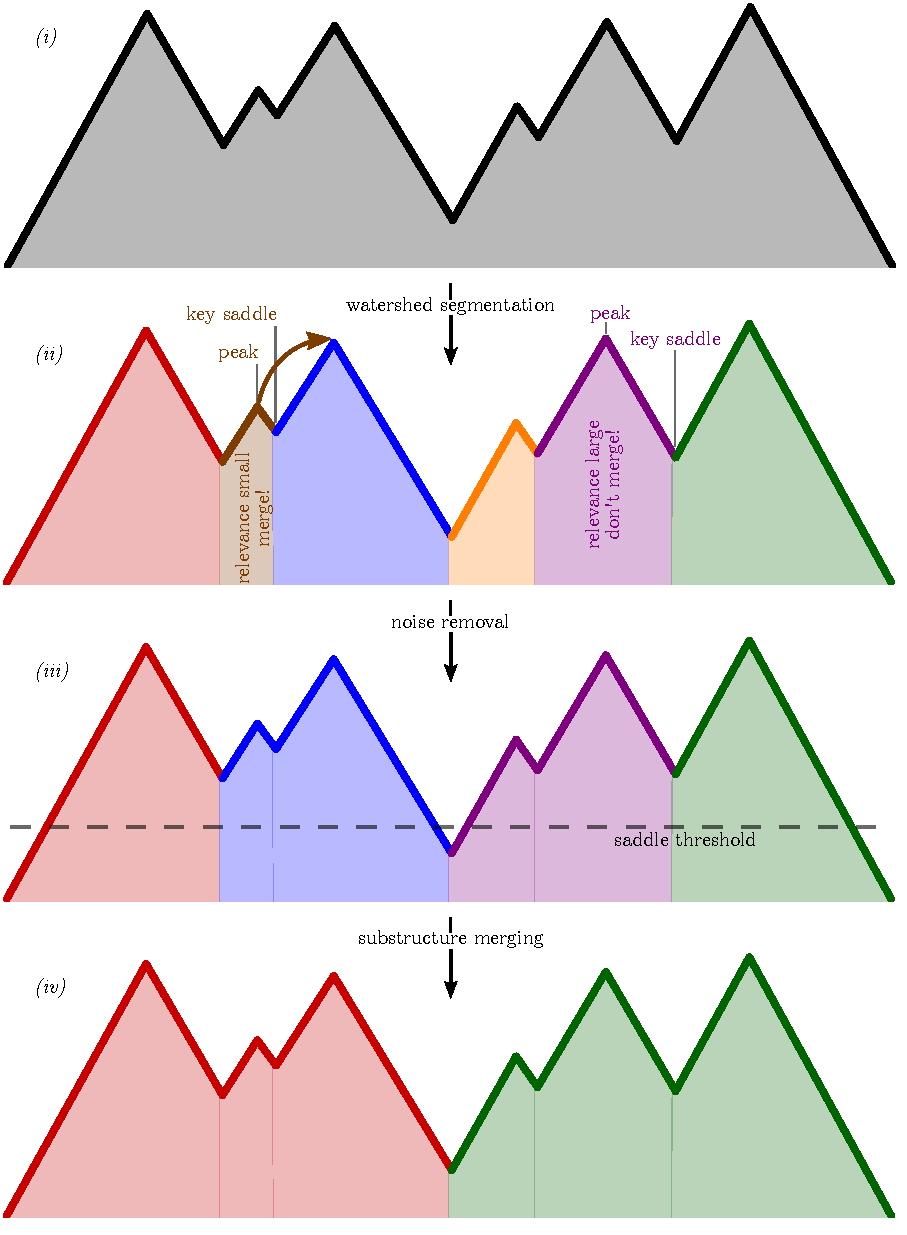
\includegraphics[height=.95\textheight]{../report/images/phew/soap.pdf}
	
	{\tiny Image adapted from \cite{PHEW}.}
\end{frame}

\section{Datasets}
\begin{frame}
	\frametitle{Test Cases}
	
	To demonstrate the effects of the particle unbinding, the following datasets will be used:
	\begin{itemize}
		\item \dt-dataset: A highly idealistic structures where the effects can be seen and evaluated more easily, created using \dice\ \parencite{DICE}.\\[.5em]
		
		\item \cosmo-dataset: A halo from the previously shown cosmological simulation which is made up from 7030 particles.
		
	\end{itemize}

%		In the \dt-dataset, each structure is initially generated as an isolated, spherically symmetric halo that follows the Navarro-Frenk-White (NFW) mass profile. 
%		The individual halos are later joined together to create one large structure that contains substructure(s).\\[.5em]
%
%		All particle masses are identical and  all particles of a clump are set to be bound to the clump.
\end{frame}



\begin{frame}
	\begin{figure}[htbp!]
		\centering
		\minipage[t]{0.497\textwidth}
		\centering
		\fbox{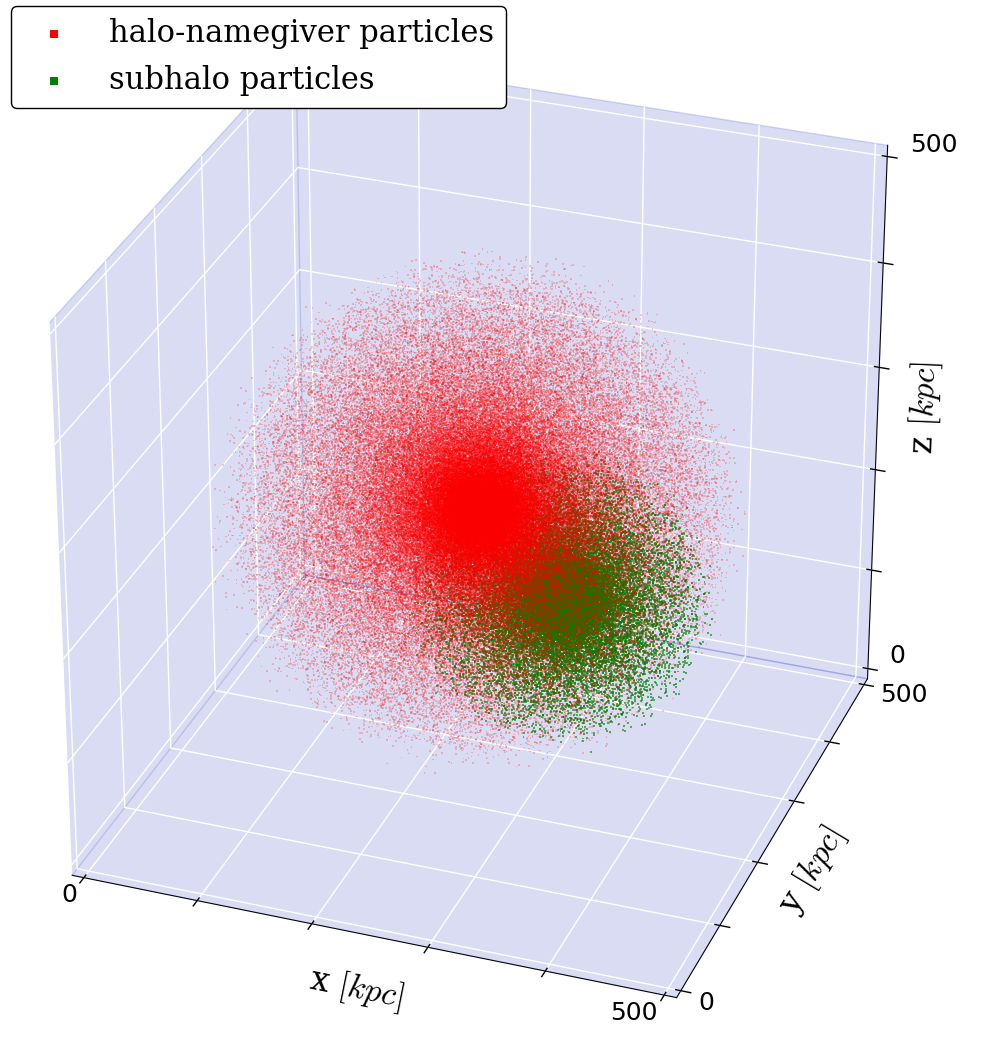
\includegraphics[height=\textwidth]{../report/images/dice-two/dice-two-original-plot.png}}%
		\caption{\footnotesize
			The initial particle distribution of the \dt\ dataset. A smaller halo (subhalo 1) made of 40'000 particles is nested within a bigger halo (halo-namegiver), which contains 200'000 particles.
		}%
		\label{fig:dice_two_origin}
		\endminipage%\hspace{.1cm}
		\hspace*{\fill}
		%
		\minipage[t]{0.497\textwidth}
		\centering
		\fbox{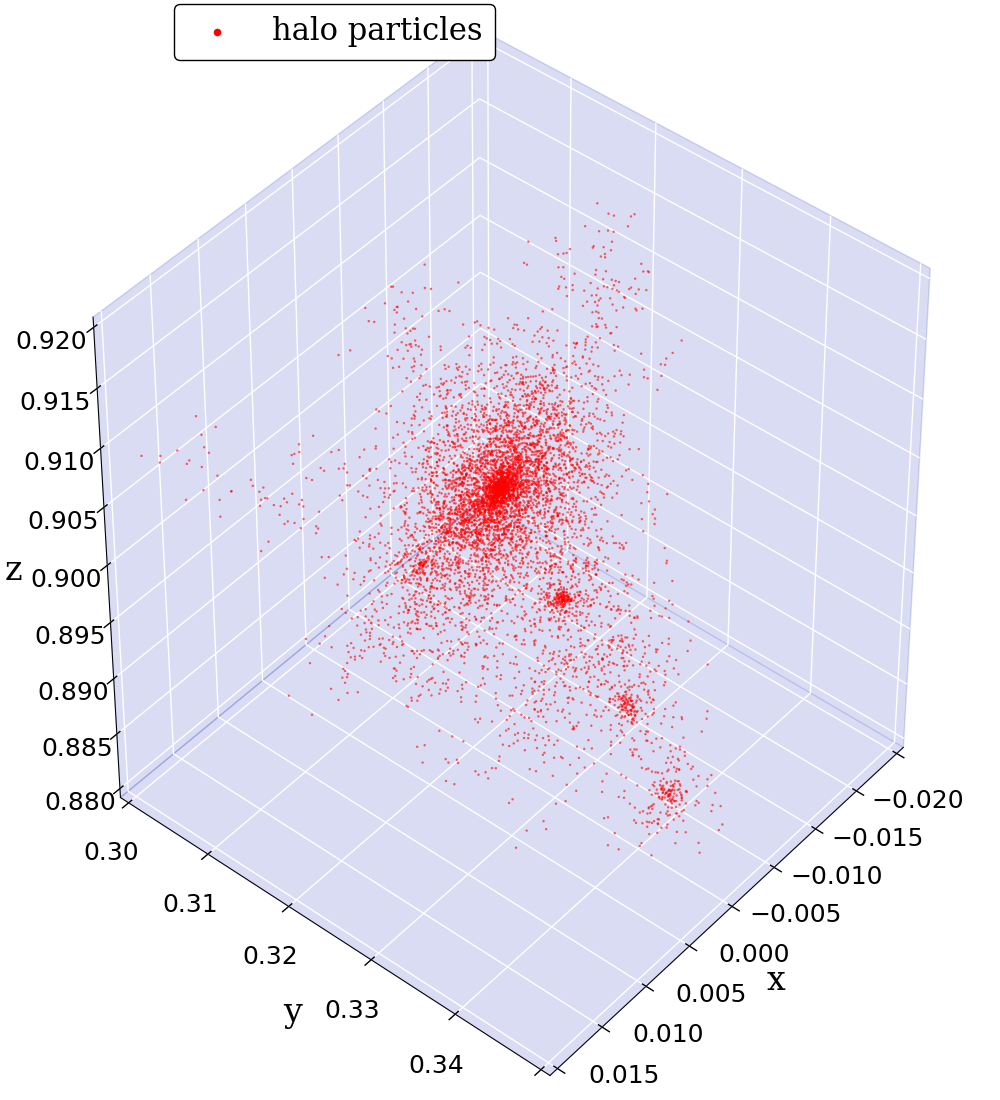
\includegraphics[height=\textwidth, keepaspectratio]{./images/cos-fullhalo-66858.png}}%
		\caption{\footnotesize
			\cosmo-dataset: A halo as identified by \phew\ of the previously shown cosmological simulation at redshift $z = 0$. 
		}%
		\label{fig:dice_sub_origin}
		\endminipage\hspace*{\fill} 
	\end{figure}
\end{frame}



%\begin{frame}
%	\frametitle{Test Cases}
%	
%	\begin{columns}
%		\column{.25\textwidth}
%		Third test case: A halo from the cosmological simulation containing  $128^3$ dark
%		matter particles at redshift $z = 0$ with $H_0 = 70.4$ and density parameters $\Omega_m = 0.272$ and $\Omega_\Lambda= 0.728$.
%		The box length corresponds to 88.8 Mpc.
%		\vfill
%		\column{.75\textwidth}
%		\begin{figure}
%			\centering
%			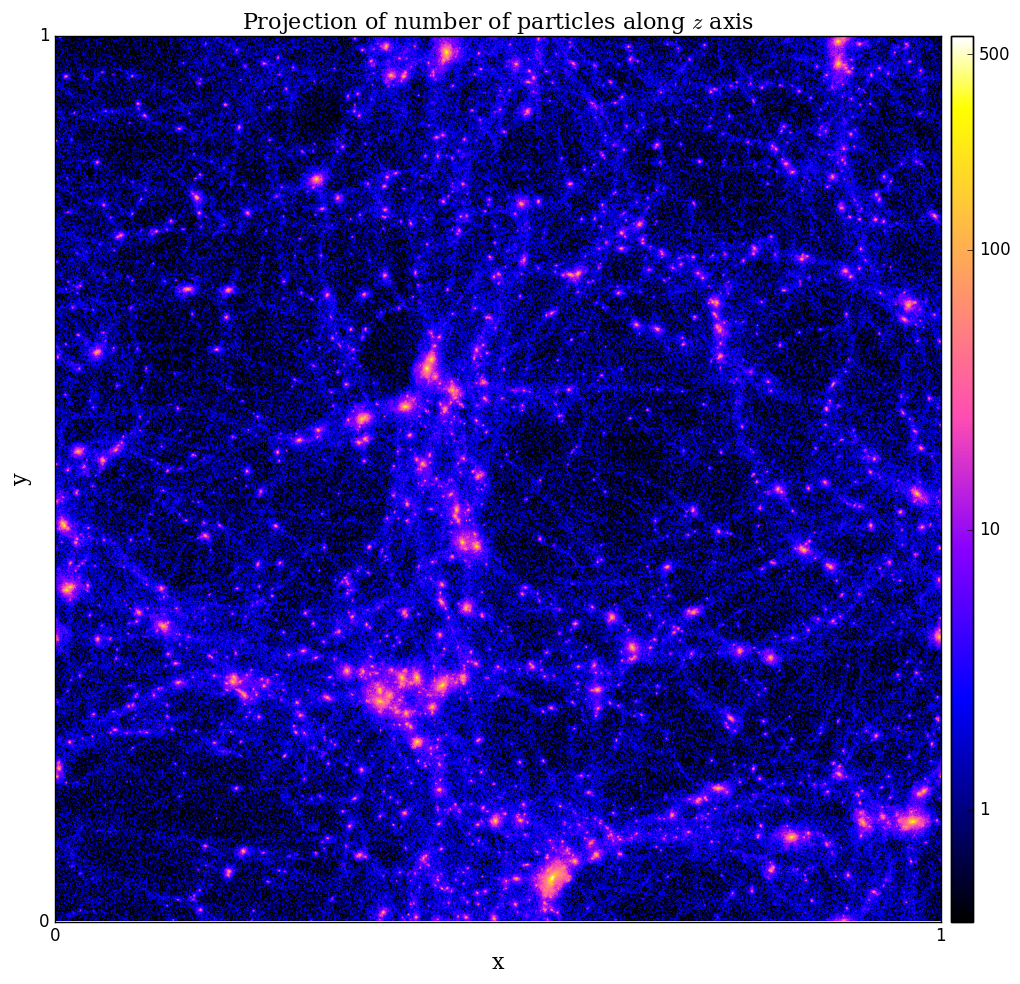
\includegraphics[width=8.2cm]{../report/images/cosmo/cos-part2map-npart.png}
%			%		\caption{
%			%		}
%		\end{figure}
%		\vfill
%	\end{columns}
%	
%\end{frame}

\section{Unbinding Particles}
\begin{frame}
	\frametitle{Particle Unbinding}
	
%	In general, one can assign every particle a total energy $E$. A particle is considered to be ``bound'' if:
%	\begin{align*}
%		E< 0
%	\end{align*}
%	
%	Considering each clump as an isolated, time independent spherical system of collisionless dark matter particles.
%	
%	In such a system the energy $E_i$ of a particle $i$ in the centre of mass frame of the clump it belongs to can be expressed as 

	In an isolated system in the centre of mass frame, each particle $i$ can be assigned an energy $E_i$:
	\begin{align*}
	E_i = T_i + V_i = \frac{1}{2} m_i \cdot v^2_i + m_i \phi (\vec{r}_i)
	\end{align*}
	
	A particle is considered bound if:
	\begin{align*}
	E_i < 0 \quad \Leftrightarrow \quad v_i < \sqrt{- 2 \cdot \phi(\vec{r}_i)}
	\end{align*}
	
\end{frame}










\begin{frame}
	\frametitle{Particle Unbinding}
	The only considered potential $\phi$ is the gravitational potential of the particles themselves. The potential is determined by the Poisson equation:
	\begin{align*}
		\Delta \phi = 4 \pi G \rho
	\end{align*}
	
	The spherically symmetric Poisson equation  can be solved analytically for $\phi$:
	%
	\begin{align*}
	\phi (r_i) &=  - G \int\limits_{r_i}^{r_{max}} \frac{M(<\tilde{r})}{\tilde{r}^2} \mathrm{d}\tilde{r}
	- G  \frac{M_{tot}}{r_{max}}
	\end{align*}
	%
	Where $M(<r) \equiv \int\limits_0^r 4 \pi \rho(\tilde{r})\tilde{r}^2 \mathrm{d}\tilde{r} $ is the mass enclosed by a sphere of radius $r$ such that the clump's total mass is enclosed by the radius $r_{max}$: $M_{tot} = M(<r_{max})$ and $G$ is the gravitational constant and $\rho$ is the density.
\end{frame}



\begin{frame}
	\frametitle{Results: \dt-dataset}
	
	\begin{tabular}{c c}
		\phewon\ 	& \simple \\[1.5em]
		%
		%	 
		{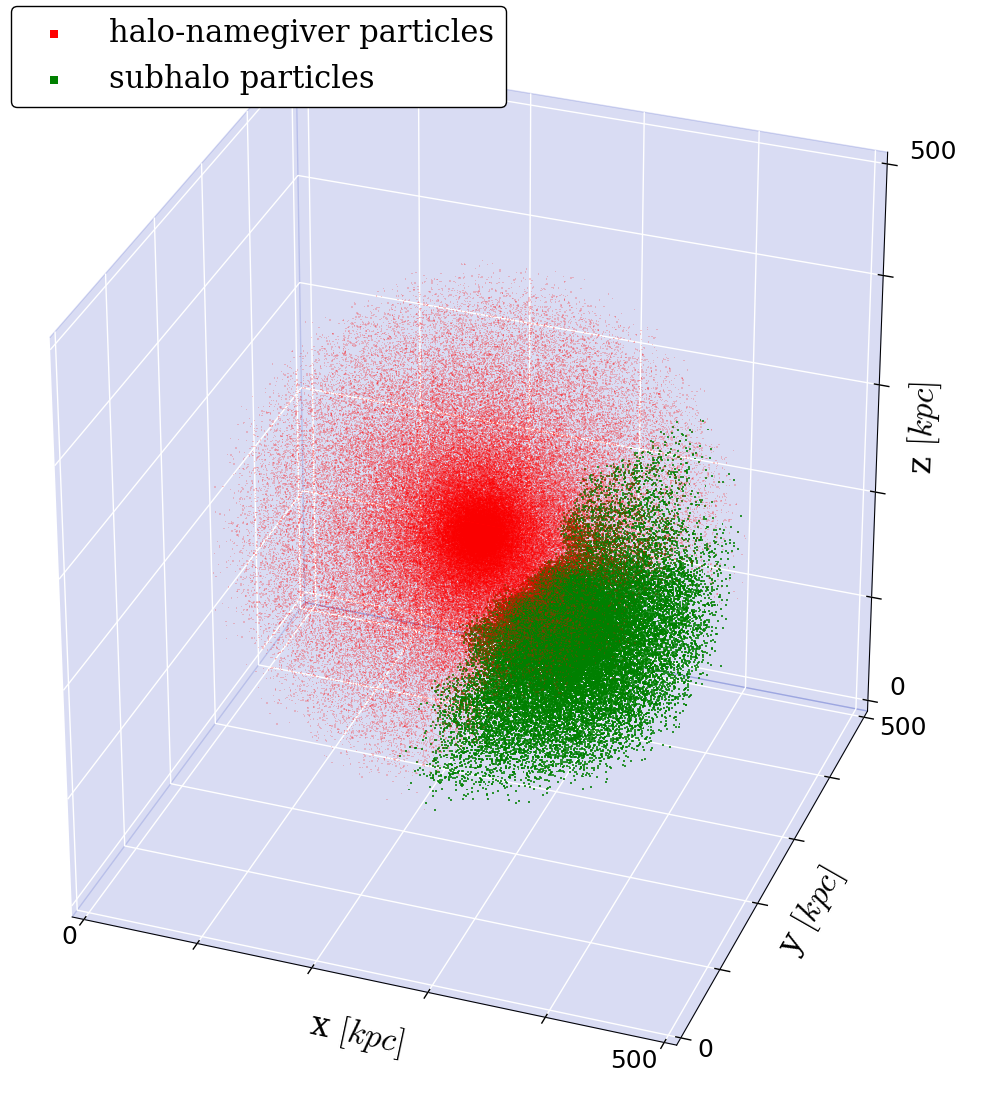
\includegraphics[width = .49\textwidth]{../report/images/dice-two/dice-two-plot-halo1451-phew.png}} \hspace*{-1em} 	& 
		{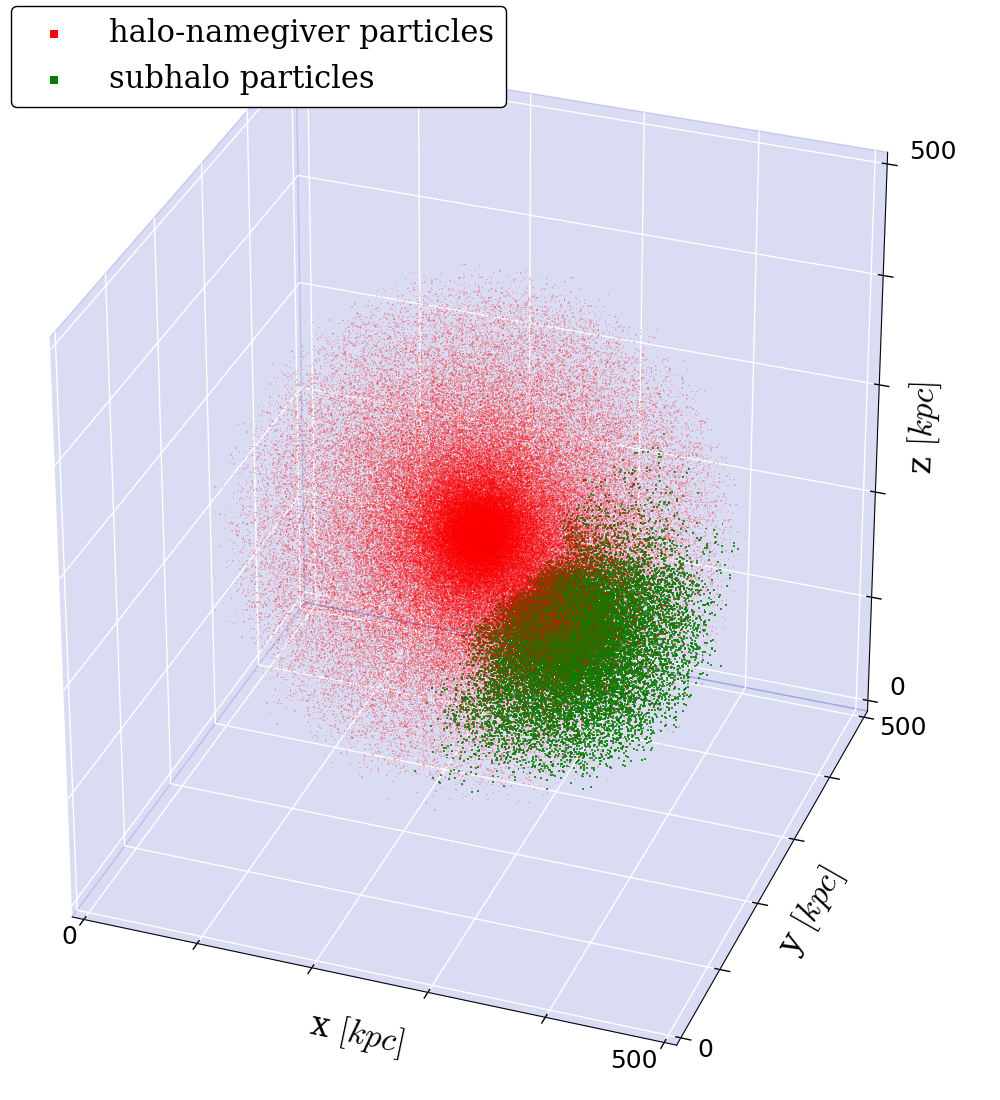
\includegraphics[width = .49\textwidth]{../report/images/dice-two/dice-two-plot-halo1451-nosaddle.png}}
	\end{tabular}
\end{frame}





\begin{frame}
	\frametitle{Results: \dt-dataset: halo-namegiver particles only}
	
	\begin{tabular}{c c}
		\phewon\ 	& \simple \\[1.5em]
		%
		%	 
		{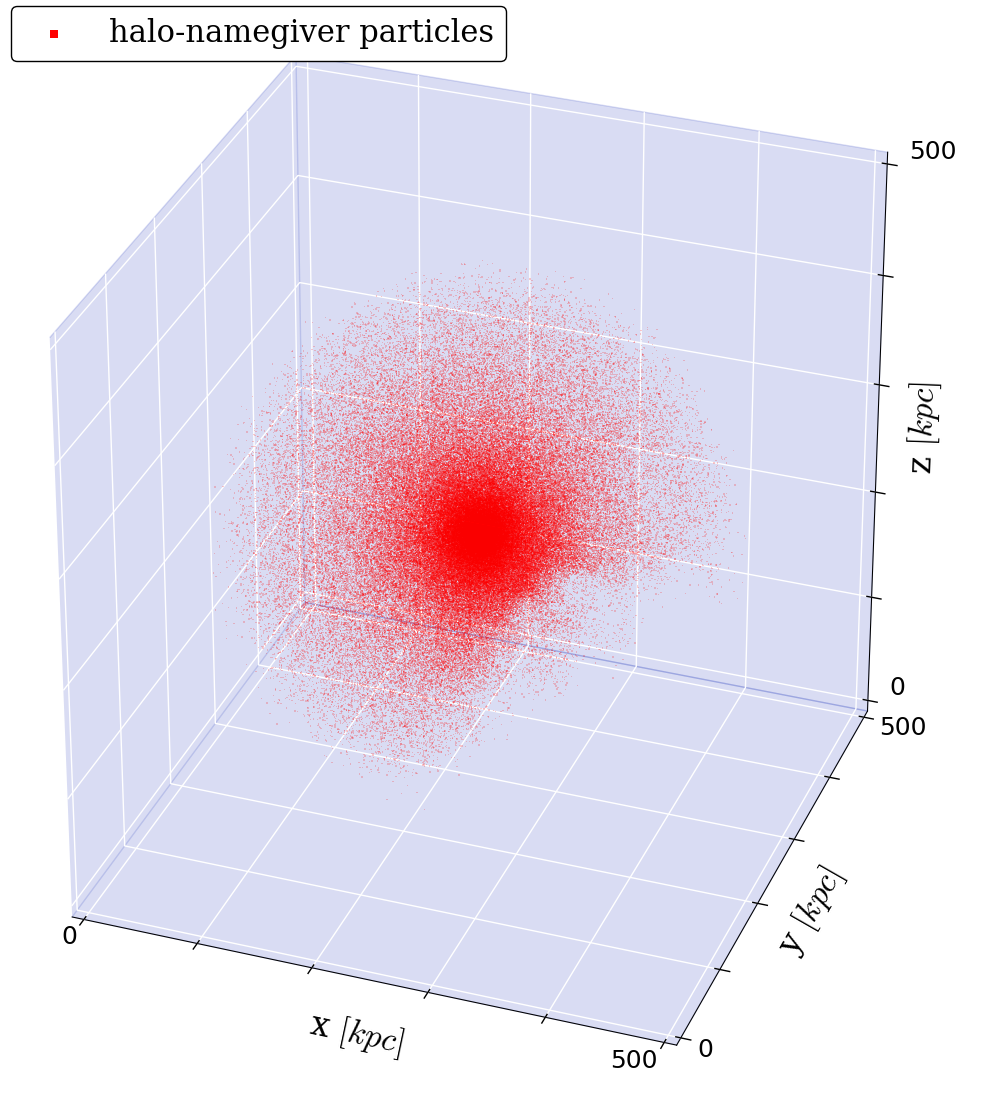
\includegraphics[width = .49\textwidth]{../report/images/dice-two/dice-two-halo-only-phew.png}} \hspace*{-1em} 	& 
		{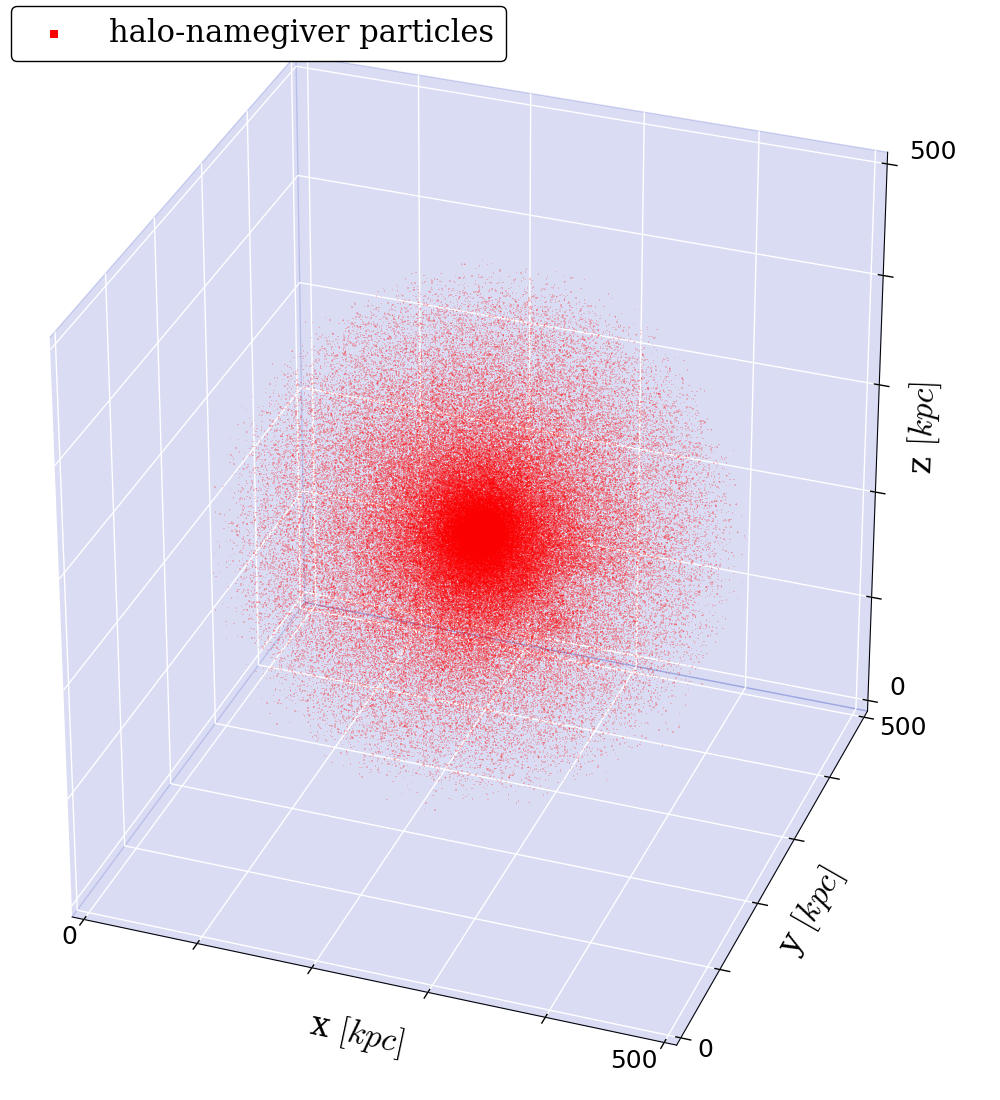
\includegraphics[width = .49\textwidth]{../report/images/dice-two/dice-two-halo-only-nosaddle.png}}
	\end{tabular}
\end{frame}




%\begin{frame}
%	\frametitle{Results: \ds-dataset}
%	
%	\begin{tabular}{c c}
%		\phewon\ 	& \simple \\[1.5em]
%		%
%		%	 
%		{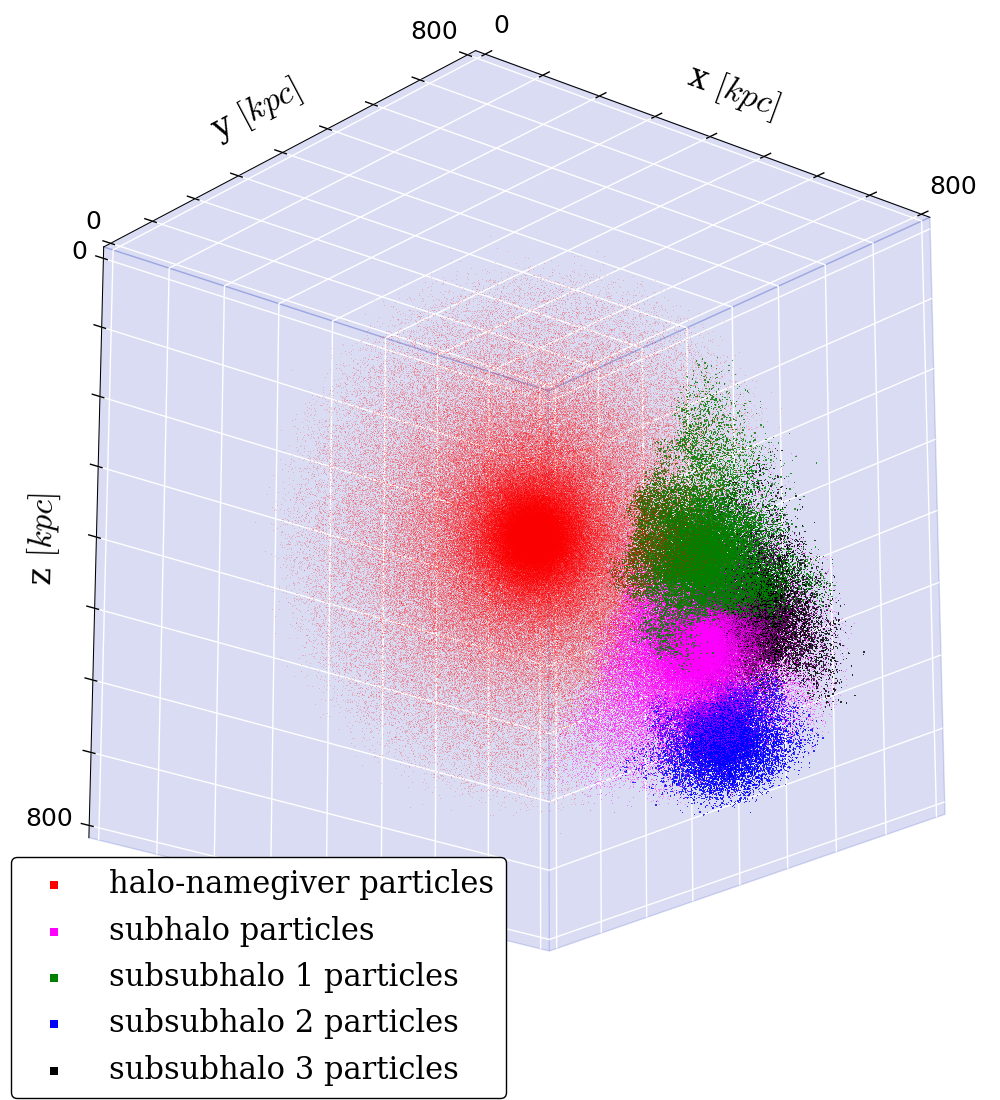
\includegraphics[width = .49\textwidth]{../report/images/dice-sub/dice-sub-plot-halo1-phew.png}} \hspace*{-1em} 	& 
%		{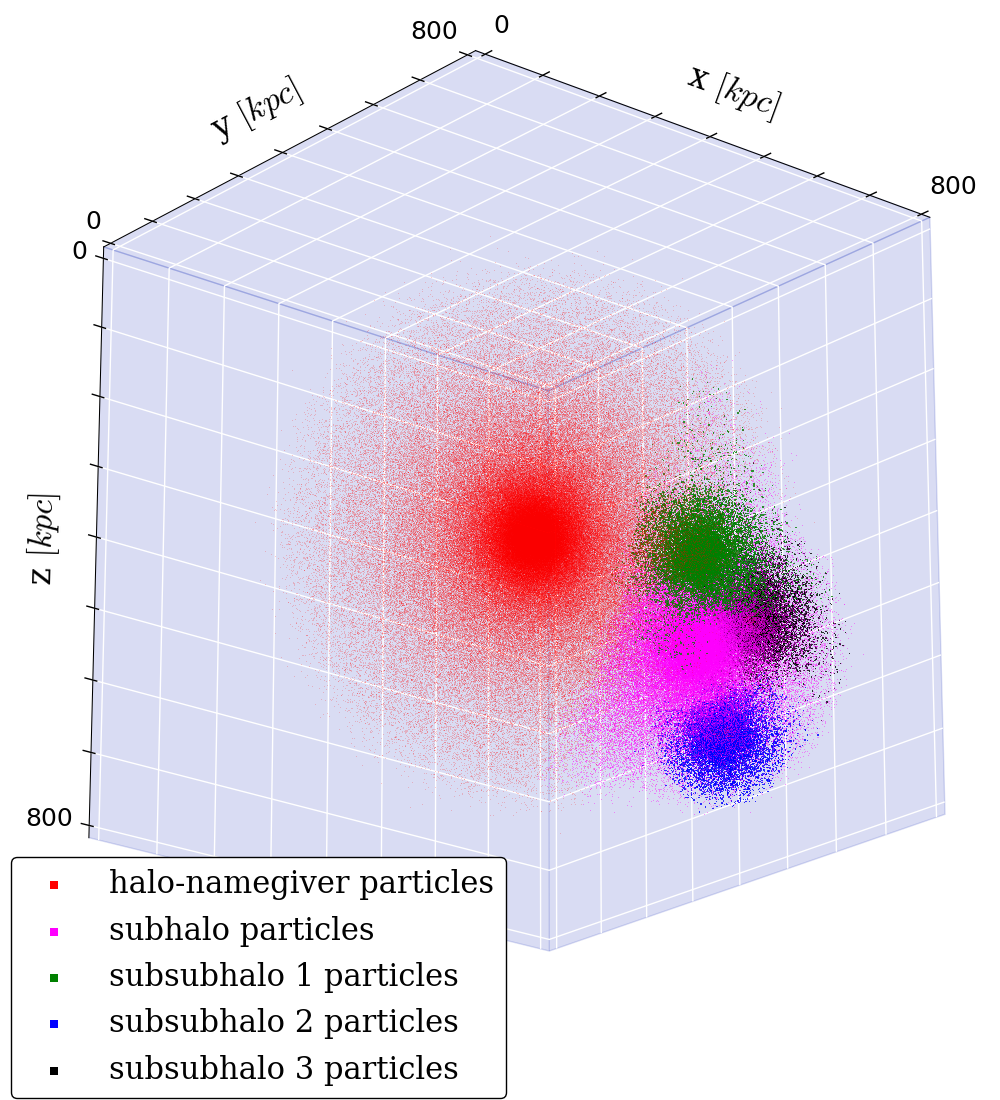
\includegraphics[width = .49\textwidth]{../report/images/dice-sub/dice-sub-plot-halo1-nosaddle.png}}
%	\end{tabular}
%\end{frame}
%
%
%
%\begin{frame}
%	\frametitle{Results: \ds-dataset: halo-namegiver particles only}
%	
%	\begin{tabular}{c c}
%		\phewon\ 	& \simple \\[1.5em]
%		%
%		%	 
%		{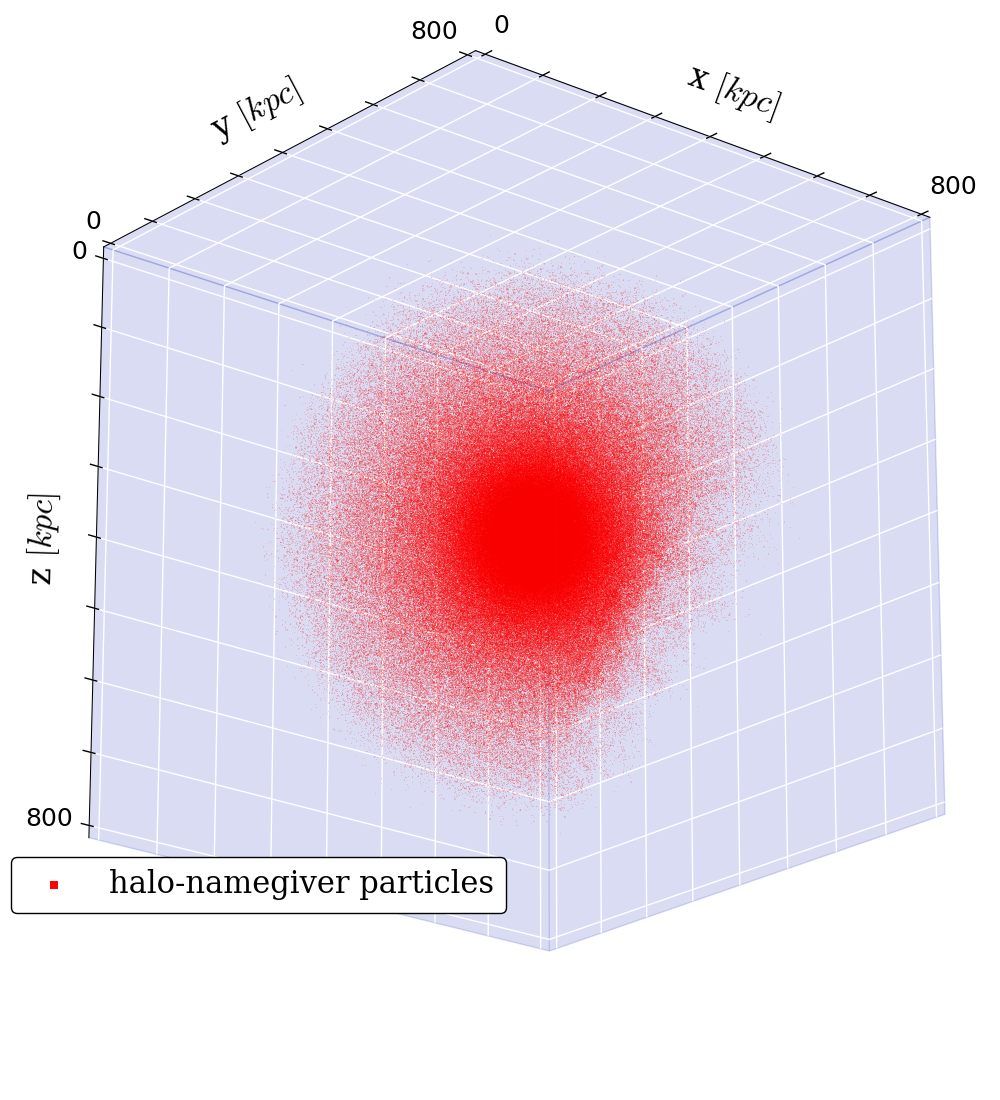
\includegraphics[width = .49\textwidth]{../report/images/dice-sub/dice-sub-halo-only-phew.png}} \hspace*{-1em} 	& 
%		{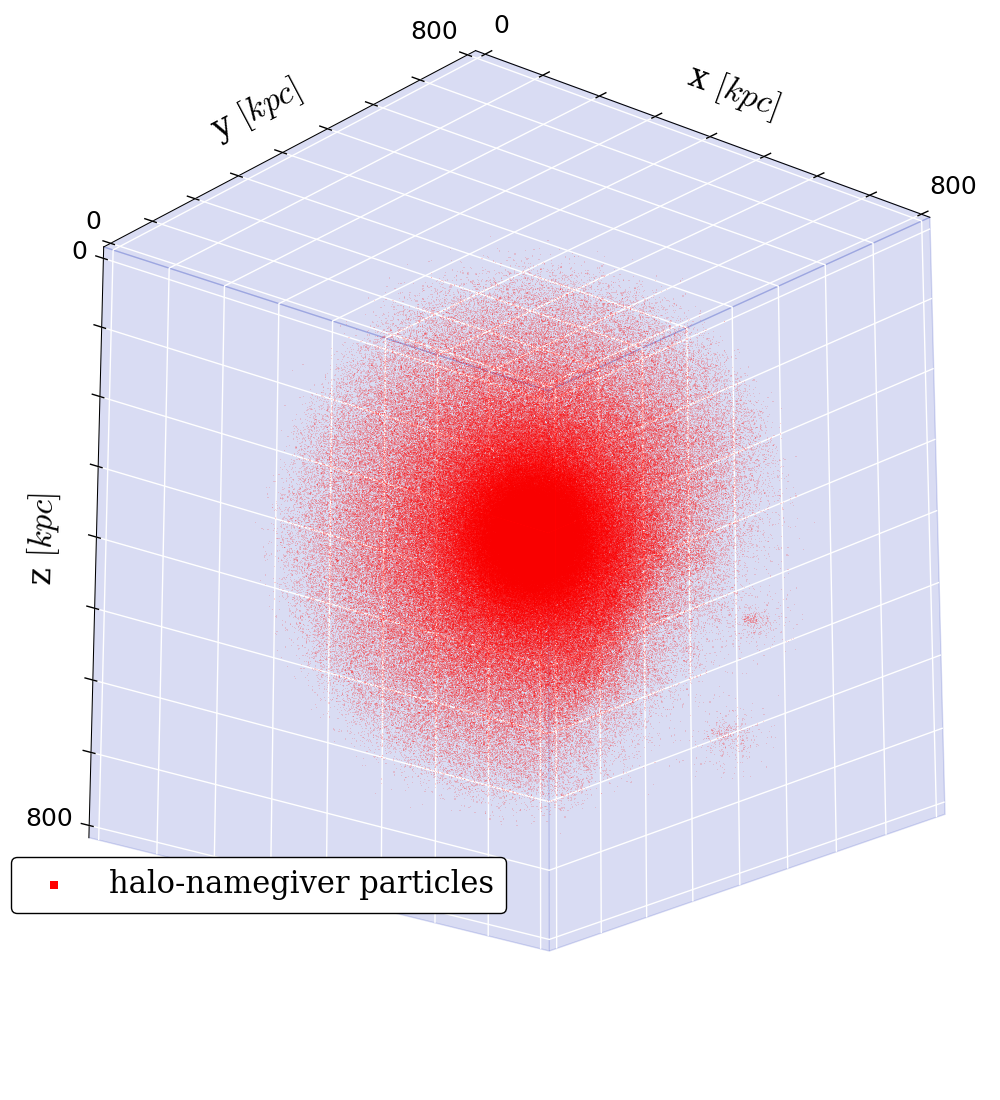
\includegraphics[width = .49\textwidth]{../report/images/dice-sub/dice-sub-halo-only-nosaddle.png}}
%	\end{tabular}
%\end{frame}



\begin{frame}
	\frametitle{Results: \cosmo-dataset: halo-namegiver particles only}
	
	\begin{tabular}{c c}
		\phewon\ 	& \simple \\[1.5em]
		%
		%	 
		{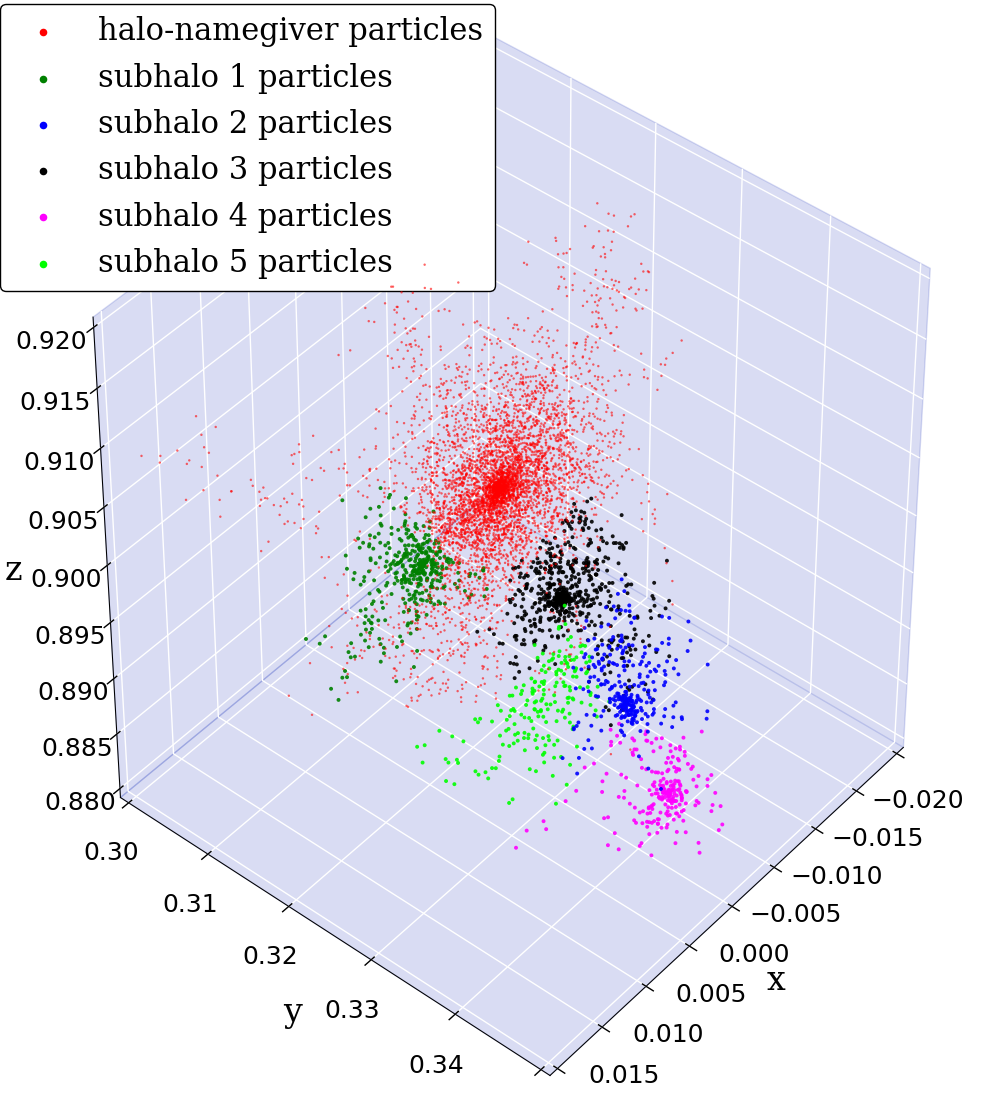
\includegraphics[width = .49\textwidth]{../report/images/cosmo/cos-halo-66858-phew.png}} \hspace*{-1em} 	& 
		{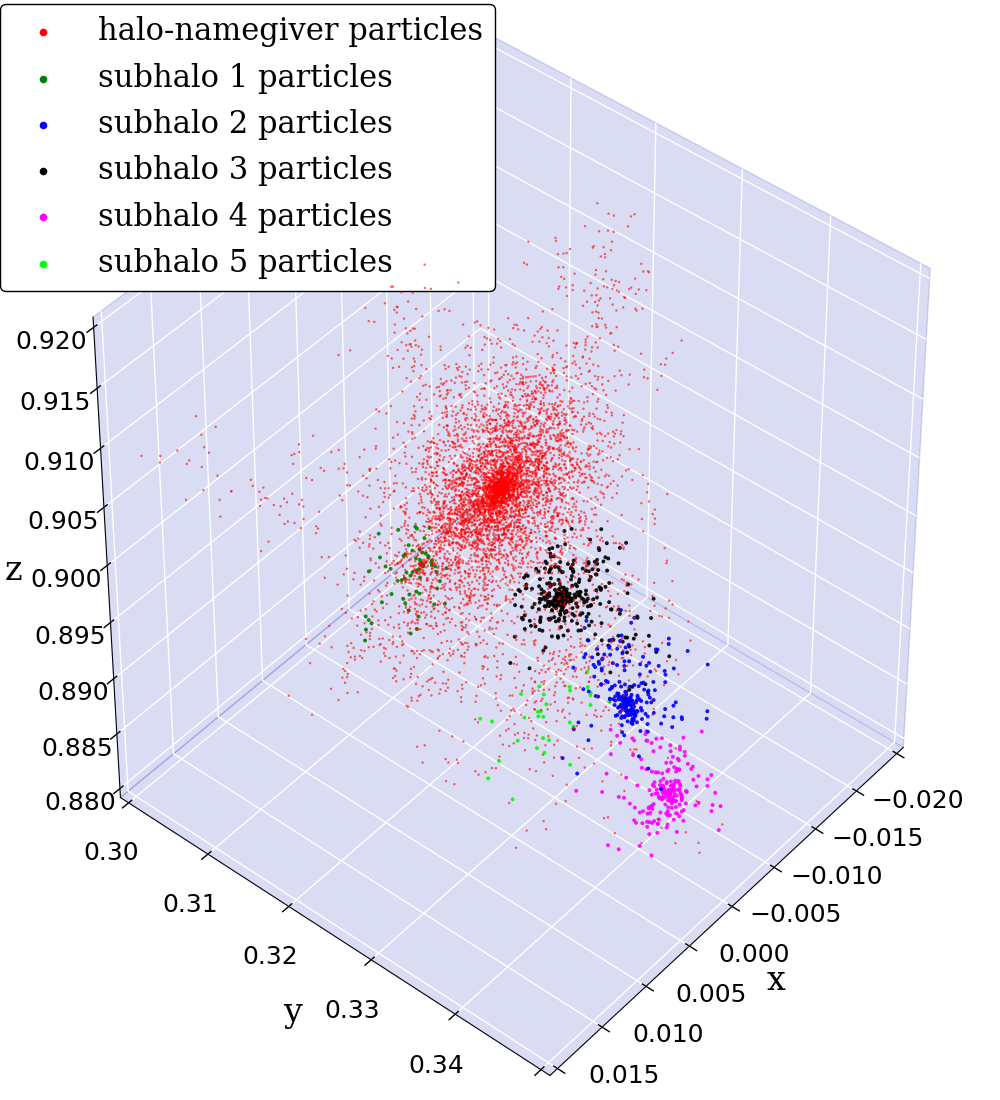
\includegraphics[width = .49\textwidth]{../report/images/cosmo/cos-halo-66858-nosaddle.png}}
	\end{tabular}
\end{frame}



\begin{frame}
	\frametitle{Results: \cosmo-dataset: halo-namegiver particles only}
	
	\begin{tabular}{c c}
		\phewon\ 	& \simple \\[1.5em]
		%
		%	 
		{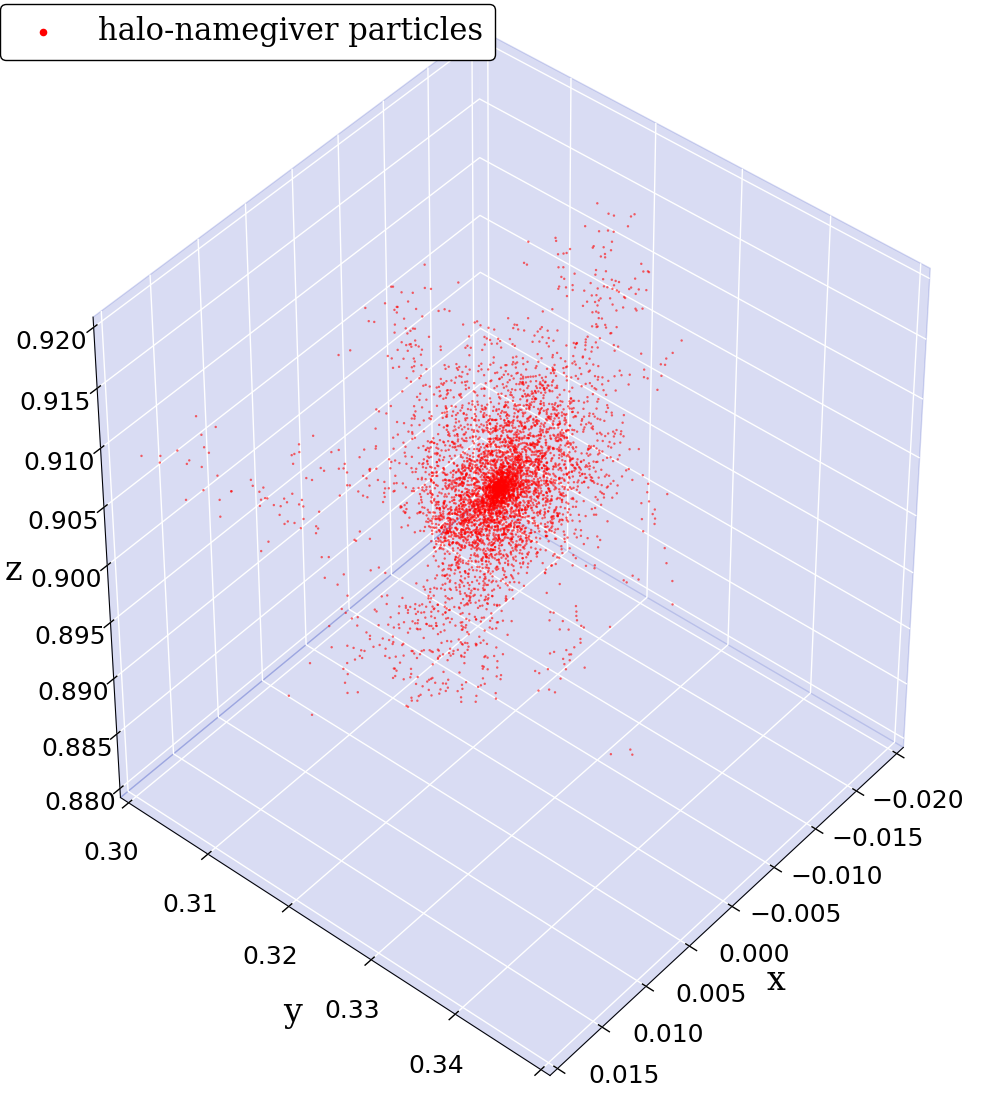
\includegraphics[width = .49\textwidth]{../report/images/cosmo/cos-halo-66858-halo-only-phew.png}} \hspace*{-1em} 	& 
		{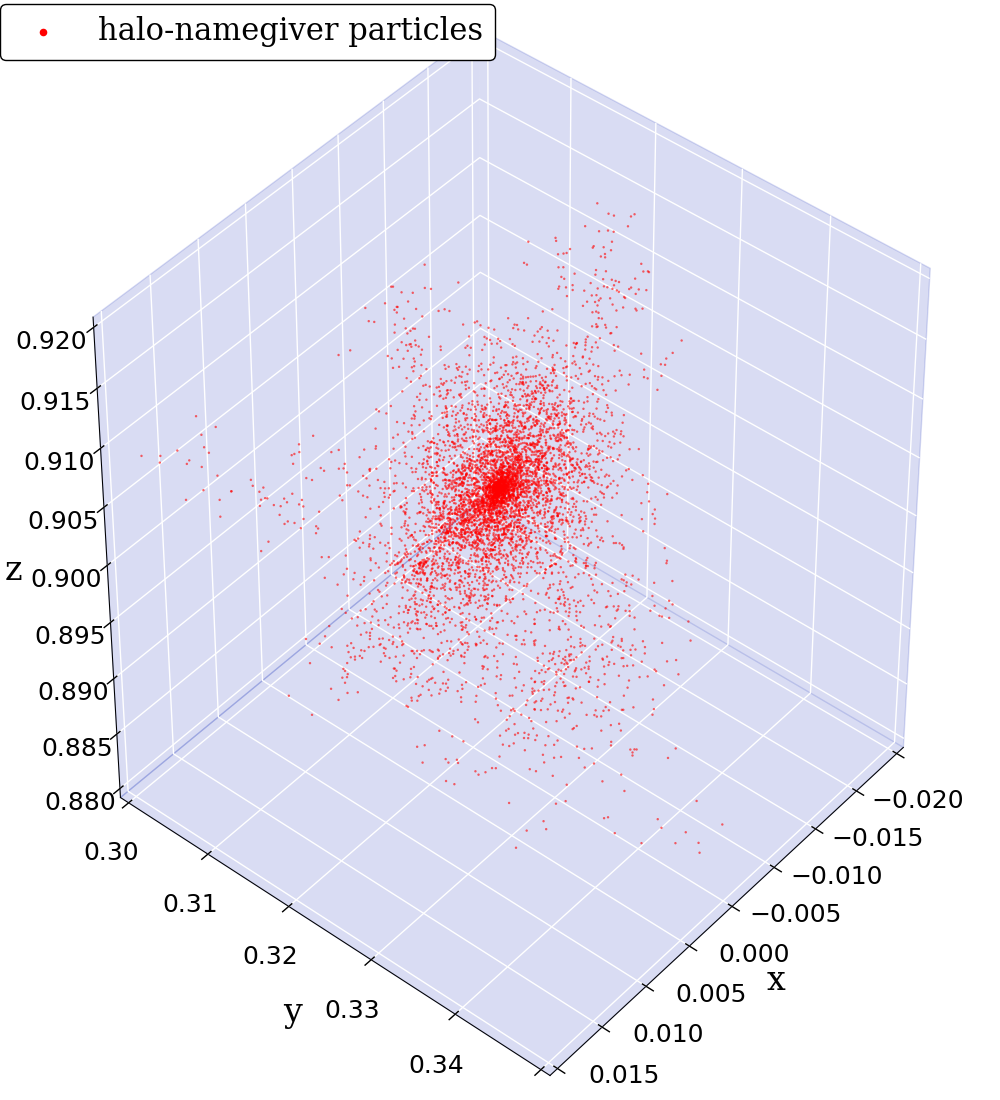
\includegraphics[width = .49\textwidth]{../report/images/cosmo/cos-halo-66858-halo-only-nosaddle.png}}
	\end{tabular}
\end{frame}

\section{Accounting for Neighbouring Structures}
\begin{frame}
	\frametitle{Accounting for Neighbouring Structures}
	
	By construction, the identified subhalos are not isolated. 
	This fact changes the situation significantly for the interpretation of what particles should be considered bound.
	
	Consider first a particle $\alpha$ in the potential of an isolated clump:
	
	
	\begin{figure}
		\centering
		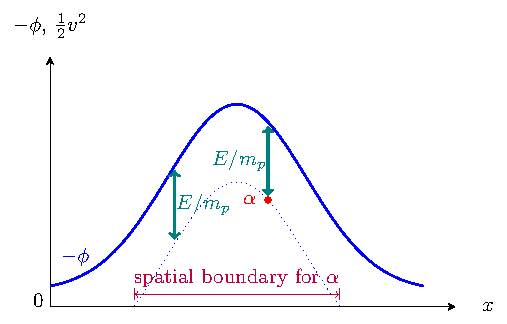
\includegraphics[width=.7\textwidth]{../report/images/tikz/boundaries.pdf}
	\end{figure}
	
	
	The spatial boundaries of its trajectory can be found by demanding energy conservation
	$	E/m_p = \frac{1}{2} v^2 + \phi = const.	$
	by following the curve of constant total energy to the points where $v^2 =0$. 
\end{frame}








\begin{frame}
	\frametitle{Accounting for Neighbouring Structures}
	
	Now apply the same thoughts to an isolated halo that is made up from two clumps:
	
	
	\begin{figure}
		\centering
		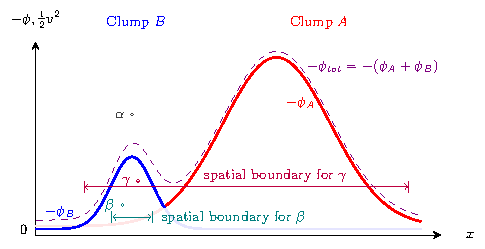
\includegraphics[width=.8\textwidth]{../report/images/tikz/potentials.pdf}
	\end{figure}
	
	\begin{itemize}
		\small
		\item $\alpha$ is clearly not bound to the clump $B$.
		\item $\beta$ will remain bound on an elliptic trajectory around the centre of mass.
		\item $\gamma$ is energetically bound to the clump just like $\beta$, but because of clump $A$'s neighbouring potential, the particle can leave the boundaries of clump $B$ and wander off deep into clump $A$.
	\end{itemize}
	

\end{frame}








\begin{frame}
	\frametitle{Accounting for Neighbouring Structures}
	
	\begin{columns}
		\column{.7\textwidth}
			$\Rightarrow$ Particles like $\gamma$ shouldn't be considered bound.
			
			The reason $\gamma$ can wander off is because its boundary extends past the interface that connects the two clumps
			
			$\Rightarrow$ the condition for a particle to be \emph{exclusively} bound must be that its trajectory must never reach that interface.
				
		\column{.3\textwidth}
			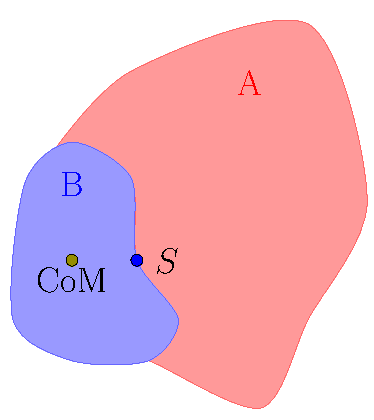
\includegraphics[width=\textwidth]{./images/tikz/saddle.pdf}
			\vspace{1cm}
	\end{columns}

	
	$\Rightarrow$ Define $S$ to be the point on the interface to the neighbouring structure(s) that is closest to B’s centre of mass and $\phi_S$ to be the potential of clump $B$ at that point. Using the same argumentation as before, a particle can't reach $S$ if 
	\begin{align*}
	v < \sqrt{ - 2(\phi - \phi_S) } 
	\end{align*}
	
\end{frame}







\begin{frame}
	\frametitle{Results: \dt-dataset}
	
	\begin{tabular}{c c}
		\simple\ 	& \neigh \\[1.5em]
		%
		%	 
		{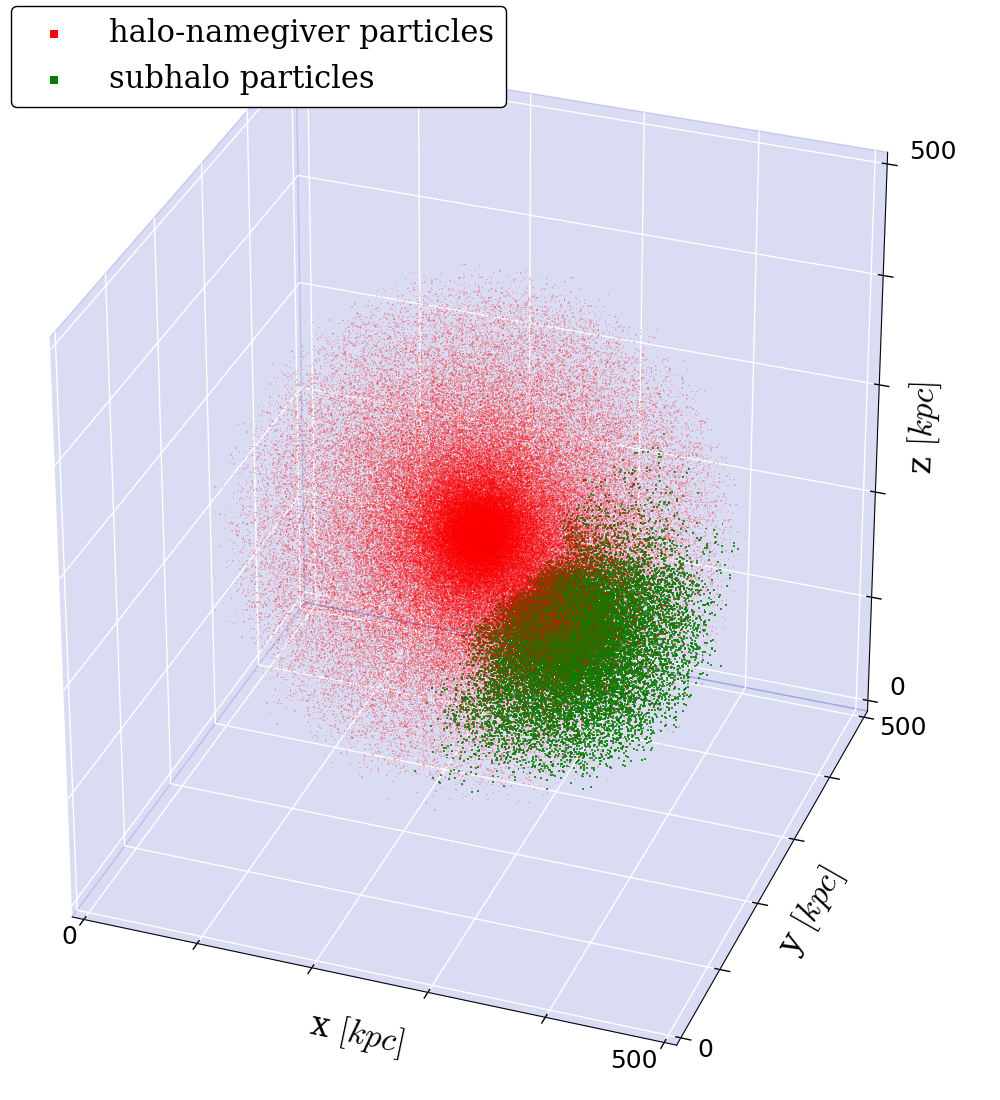
\includegraphics[width = .49\textwidth]{../report/images/dice-two/dice-two-plot-halo1451-nosaddle.png}} &
		{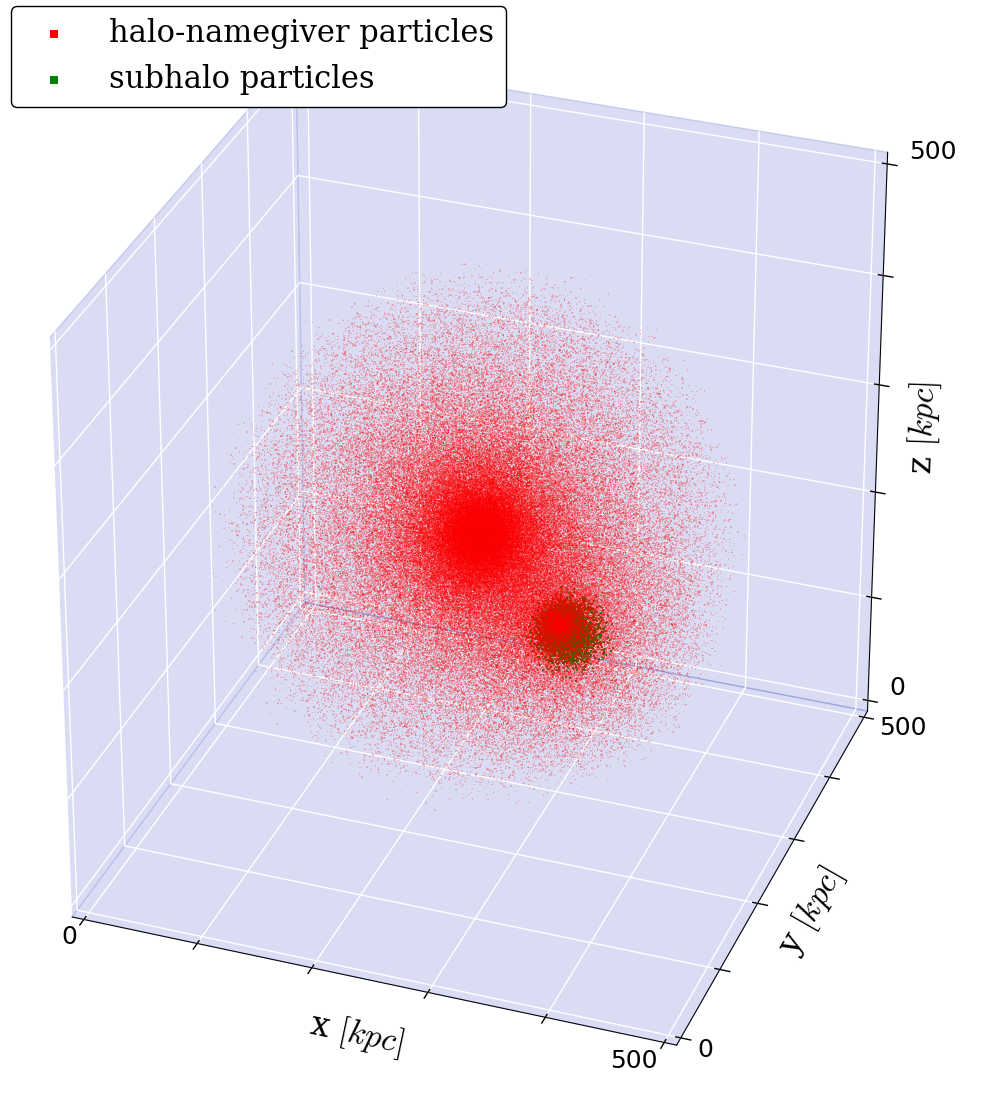
\includegraphics[width = .49\textwidth]{../report/images/dice-two/dice-two-plot-halo1451-saddle.png}} \hspace*{-1em} 
	\end{tabular}
\end{frame}





\begin{frame}
	\frametitle{Results: \dt-dataset: subhalo particles only}
	
	\begin{tabular}{c c}
		\simple\ 	& \neigh \\[1.5em]
		%
		%	 
		{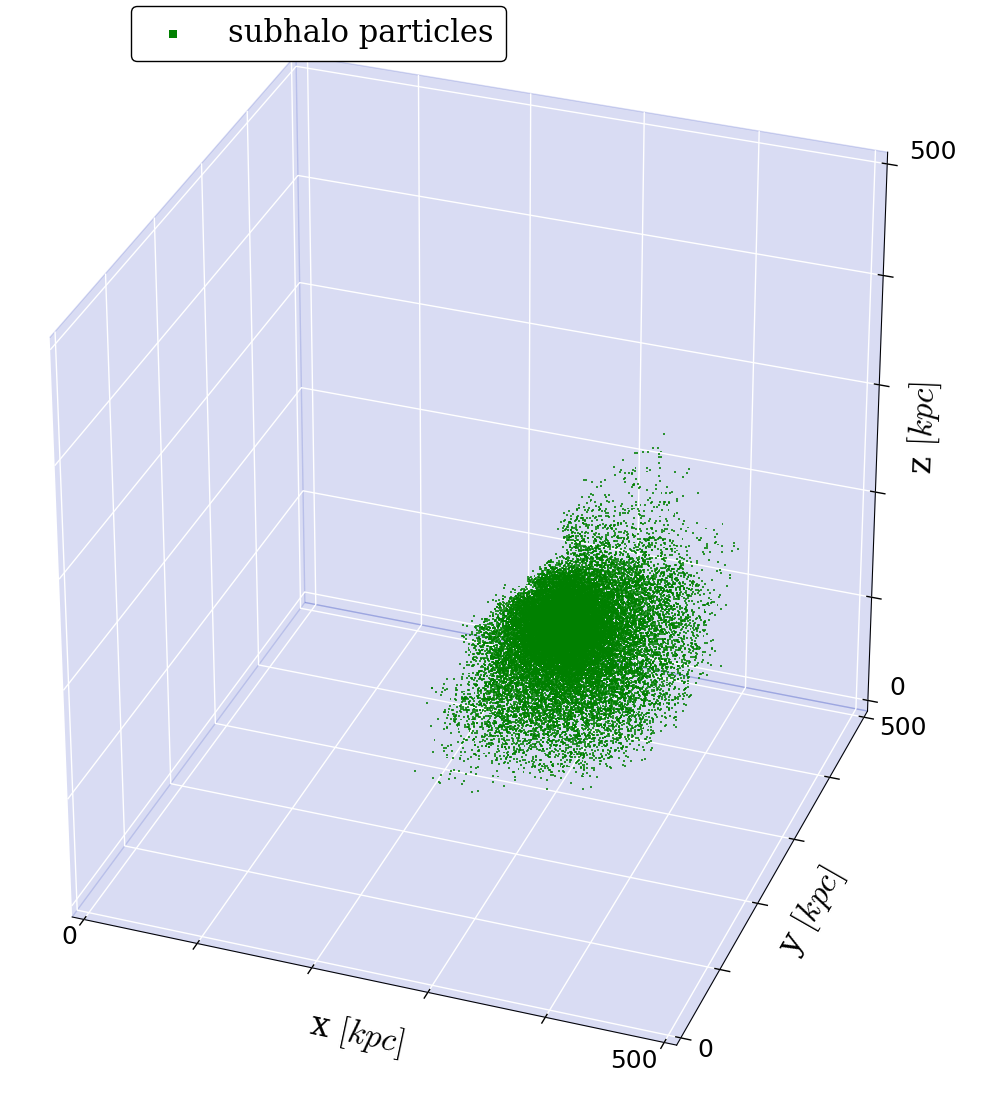
\includegraphics[width = .49\textwidth]{../report/images/dice-two/dice-two-plot-subhalo-nosaddle.png}}	&
		{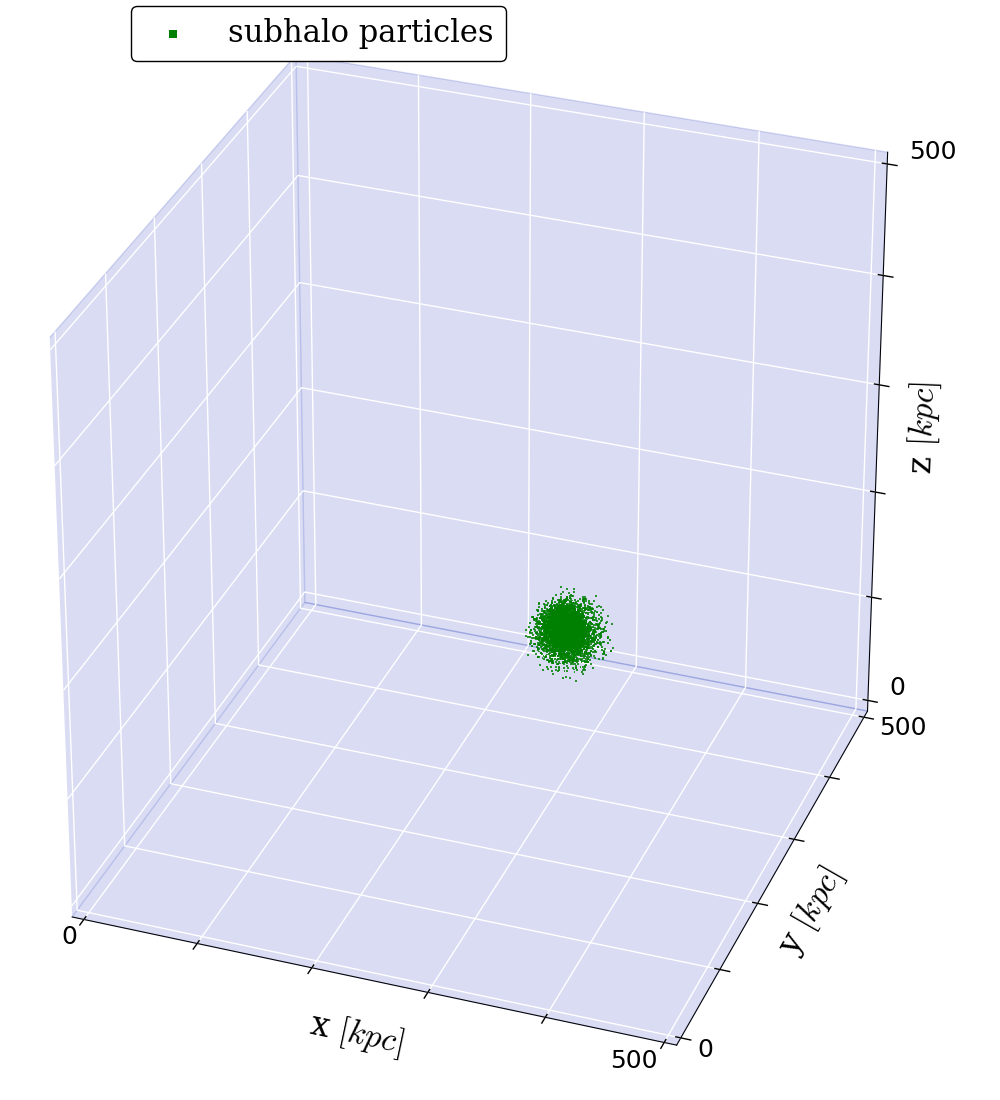
\includegraphics[width = .49\textwidth]{../report/images/dice-two/dice-two-plot-subhalo-saddle.png}}  
	\end{tabular}
\end{frame}




%\begin{frame}
%	\frametitle{Results: \ds-dataset}
%	
%	\begin{tabular}{c c}
%		\simple\ 	& \neigh \\[1.5em]
%		%
%		%
%		 
%		{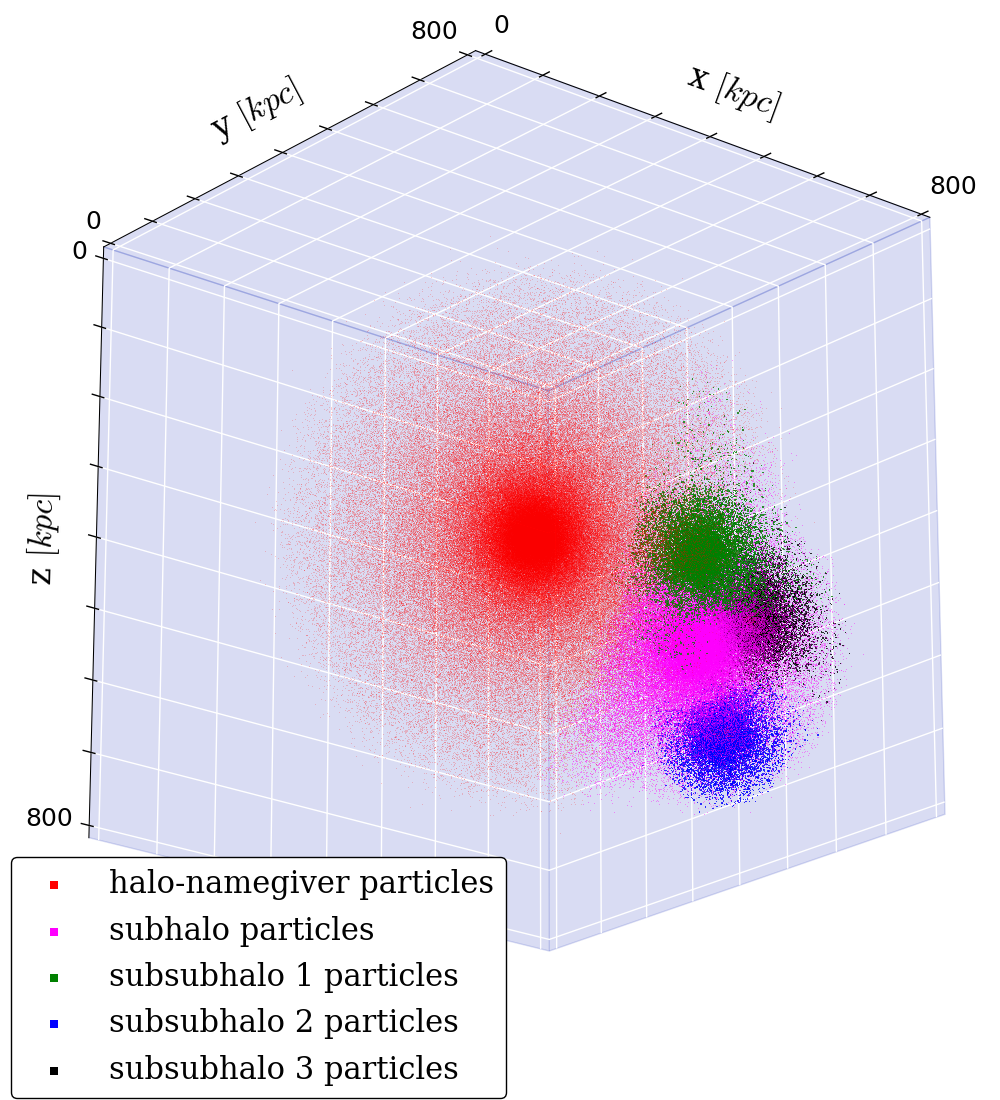
\includegraphics[width = .49\textwidth]{../report/images/dice-sub/dice-sub-plot-halo1-nosaddle.png}}	&		 
%		{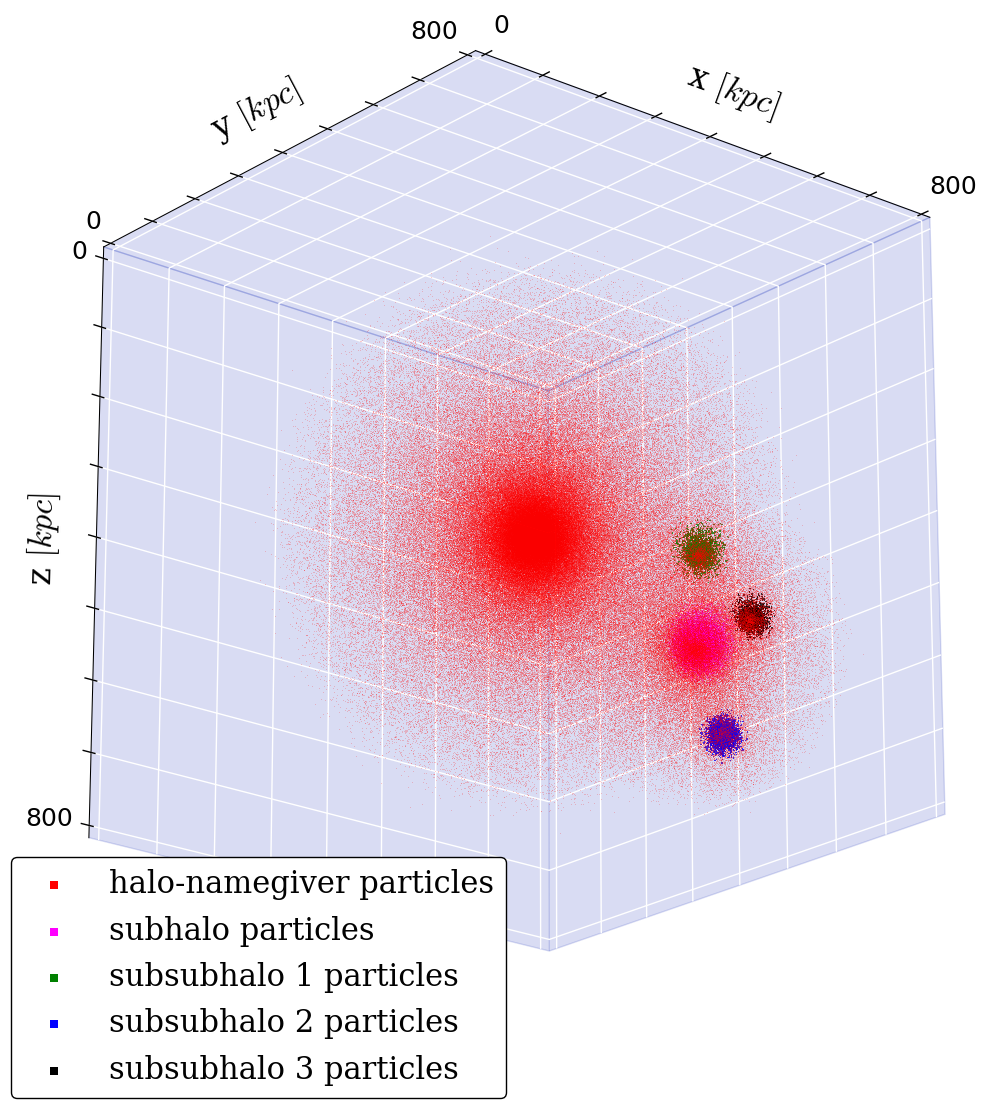
\includegraphics[width = .49\textwidth]{../report/images/dice-sub/dice-sub-plot-halo1-saddle.png}} 	
%	\end{tabular}
%\end{frame}
%
%
%
%\begin{frame}
%	\frametitle{Results: \ds-dataset: halo-namegiver particles only}
%	
%	\begin{tabular}{c c}
%		\simple\ 	& \neigh \\[1.5em]
%		%
%		%	 
%		{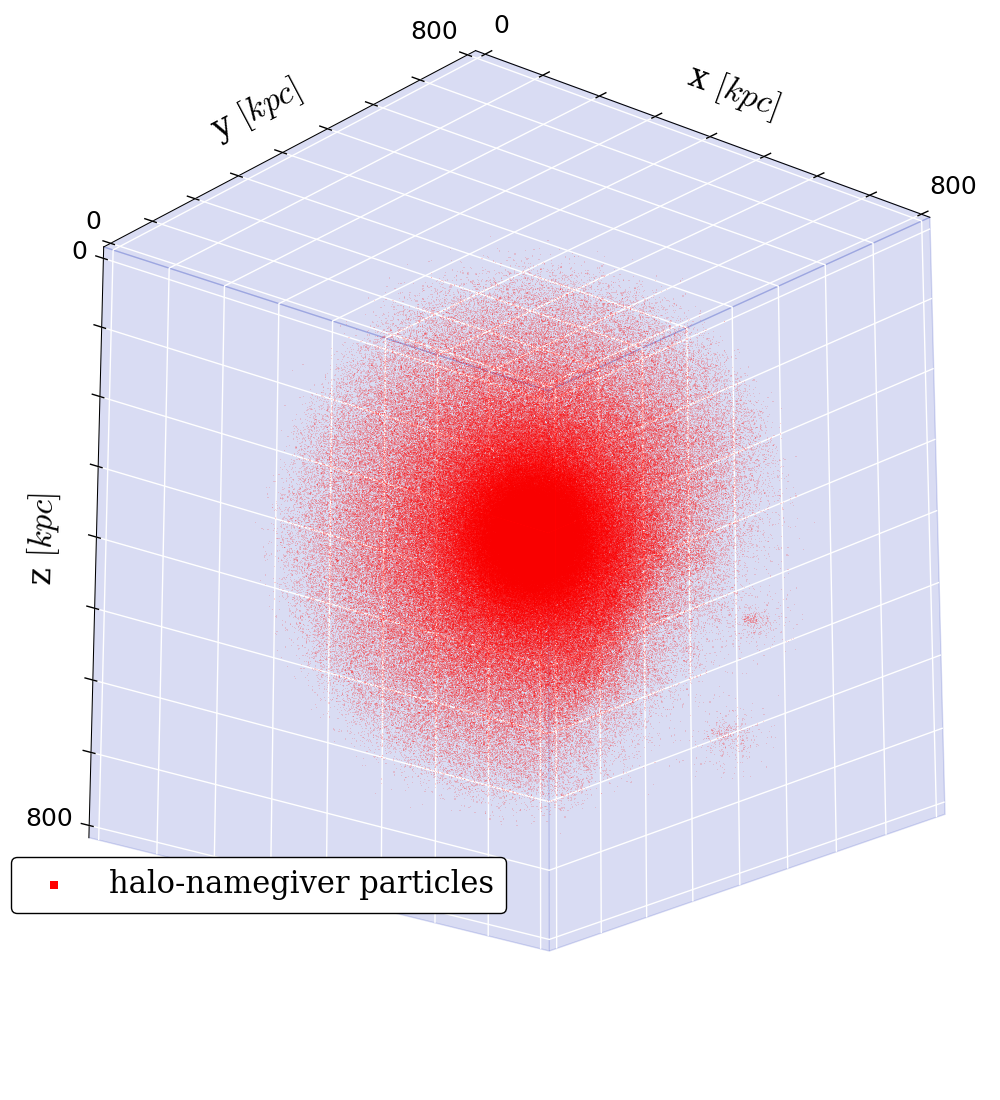
\includegraphics[width = .49\textwidth]{../report/images/dice-sub/dice-sub-halo-only-nosaddle.png}} \hspace*{-1em} 	& 
%		{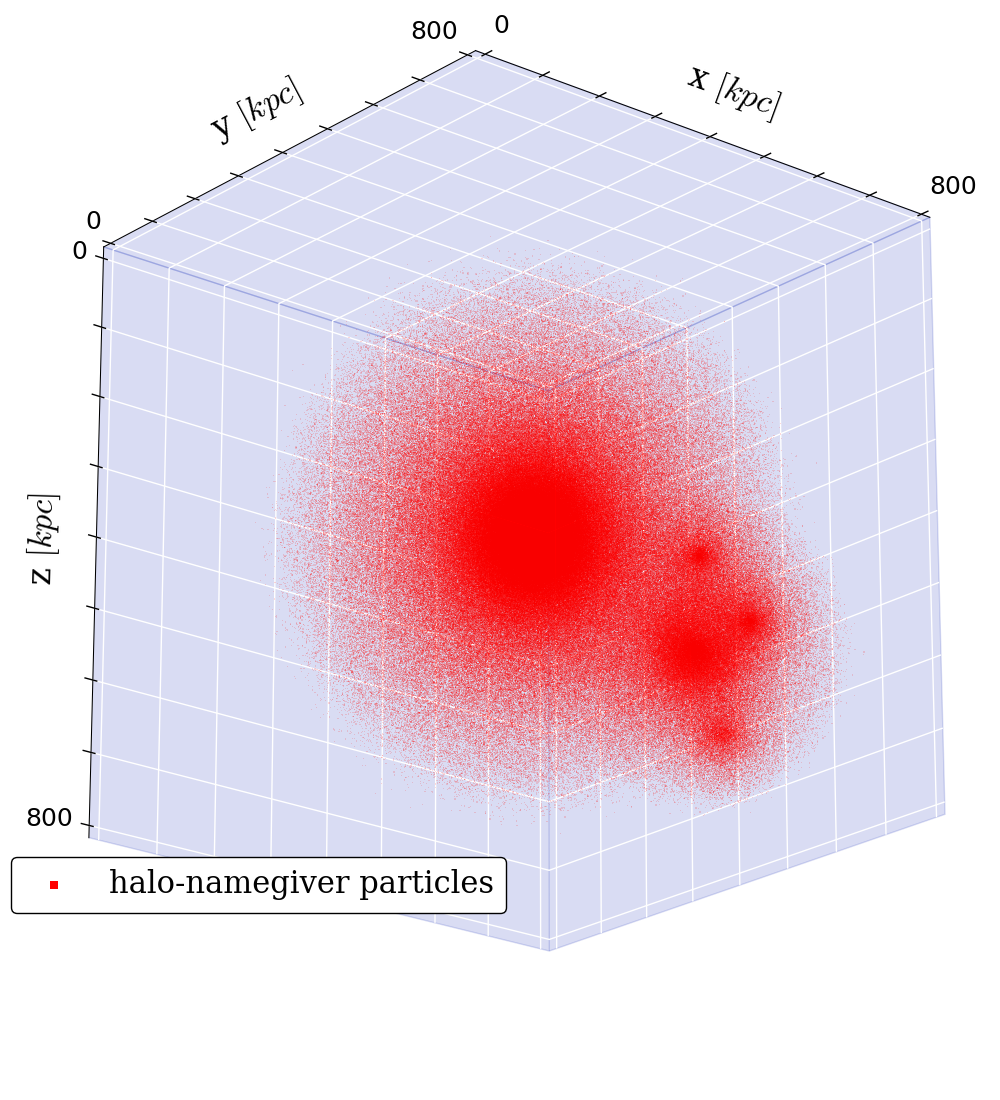
\includegraphics[width = .49\textwidth]{../report/images/dice-sub/dice-sub-halo-only-saddle.png}}
%	\end{tabular}
%\end{frame}



\begin{frame}
	\frametitle{Results: \cosmo-dataset}
	
	\begin{tabular}{c c}
		\simple\ 	& \neigh \\[1.5em]
		%
		%	 
		{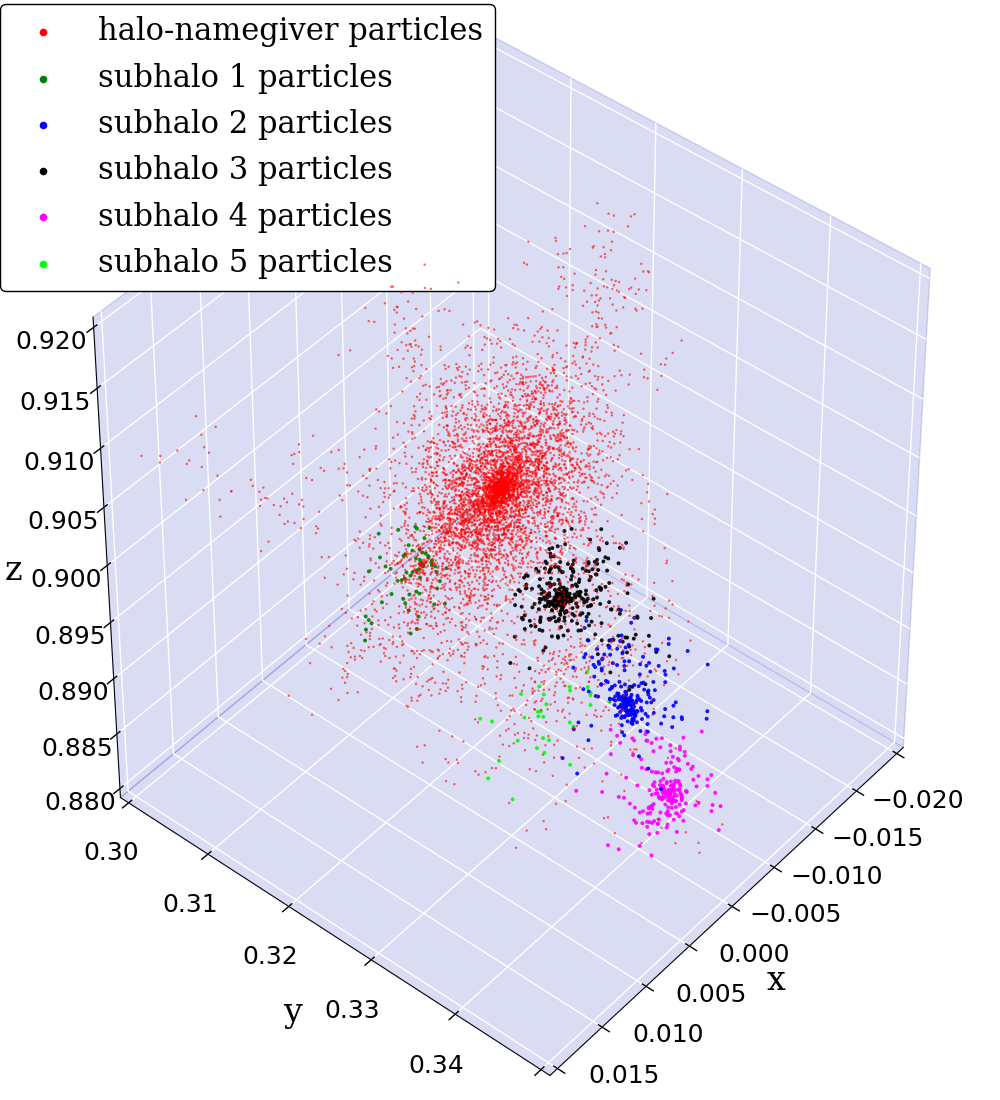
\includegraphics[width = .49\textwidth]{../report/images/cosmo/cos-halo-66858-nosaddle.png}}	& 
		{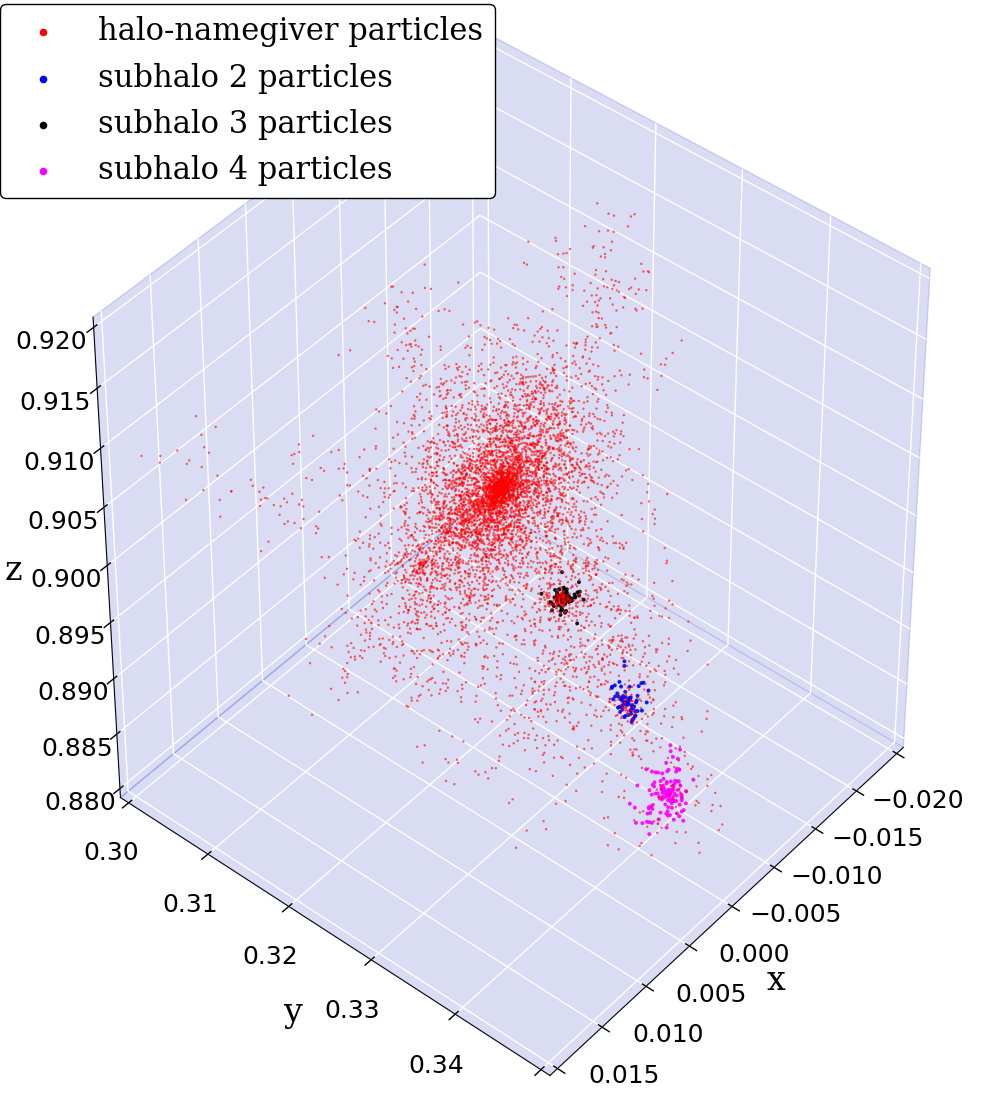
\includegraphics[width = .49\textwidth]{../report/images/cosmo/cos-halo-66858-saddle.png}}
	\end{tabular}
\end{frame}



\begin{frame}
	\frametitle{Results: \cosmo-dataset: subhalo particles only}
	
	\begin{tabular}{c c}
		\simple\ 	& \neigh \\[1.5em]
		%
		%	 
		{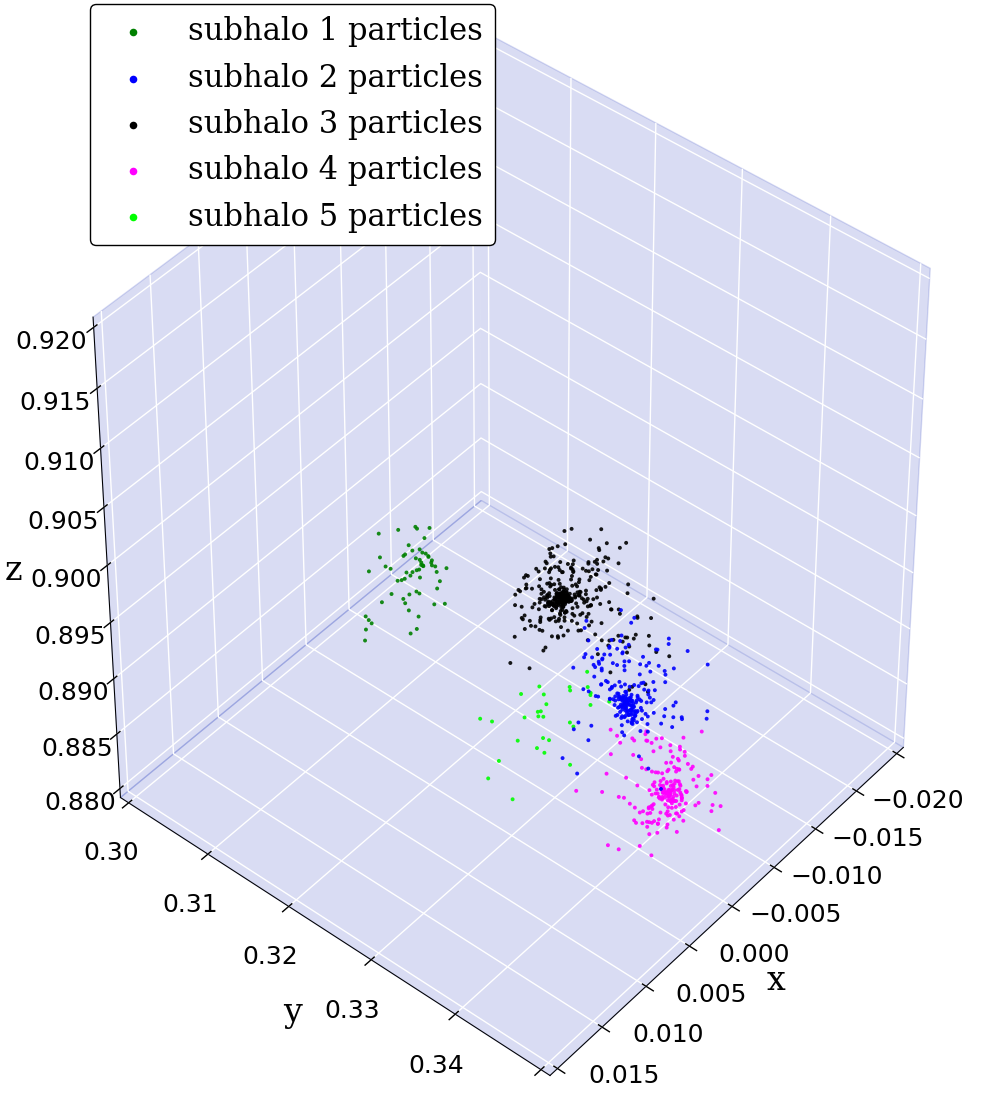
\includegraphics[width = .49\textwidth]{../report/images/cosmo/cos-halo-66858-subhalo-only-nosaddle.png}} \hspace*{-1em} 	& 
		{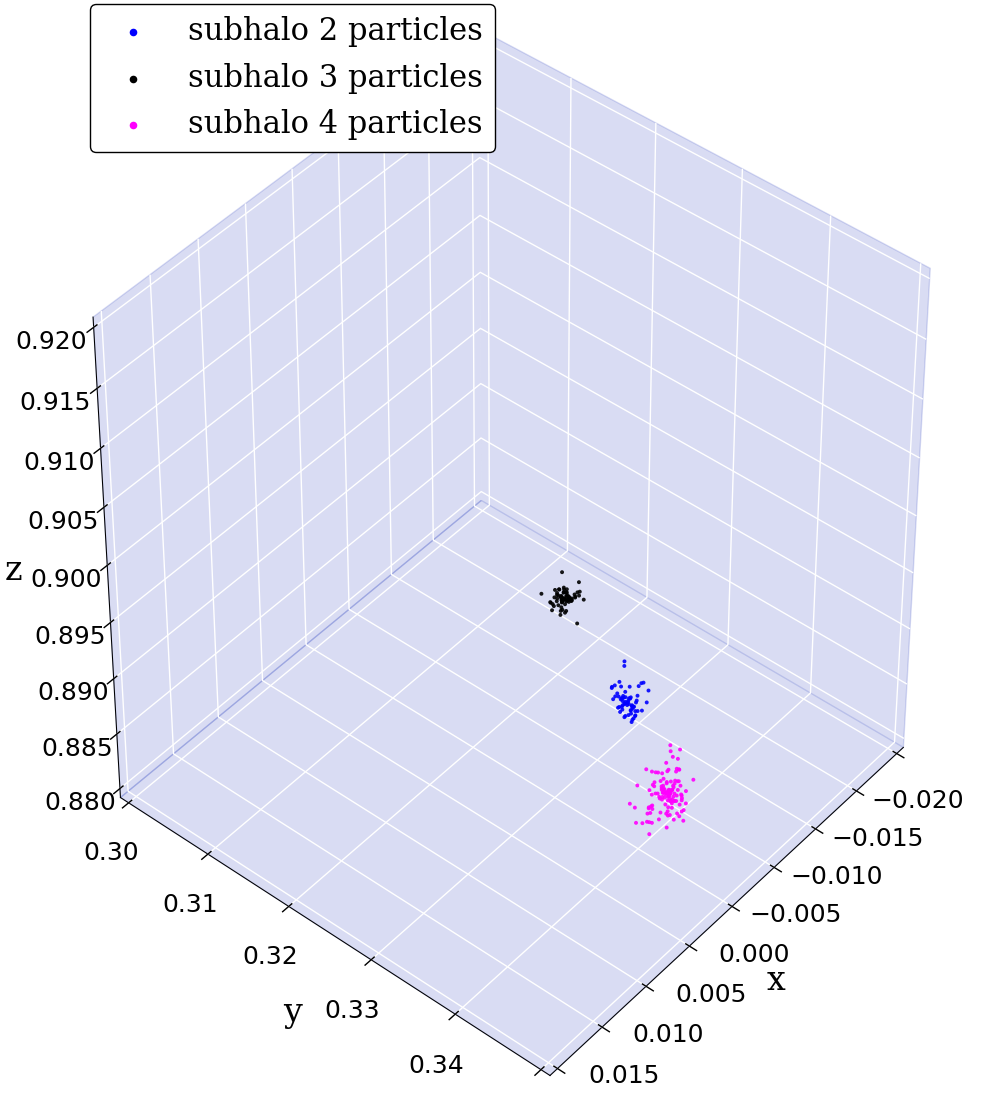
\includegraphics[width = .49\textwidth]{../report/images/cosmo/cos-halo-66858-subhalo-only-saddle.png}}
	\end{tabular}
\end{frame}

\section{Iterative Clump Property Determination}
\begin{frame}
	\frametitle{Biased Clump Properties}
	\begin{center}
		\begin{tabular}{c c}
			initial set-up 	& clumps found by \phew\ \\[.5em]
			%
			%	 
			{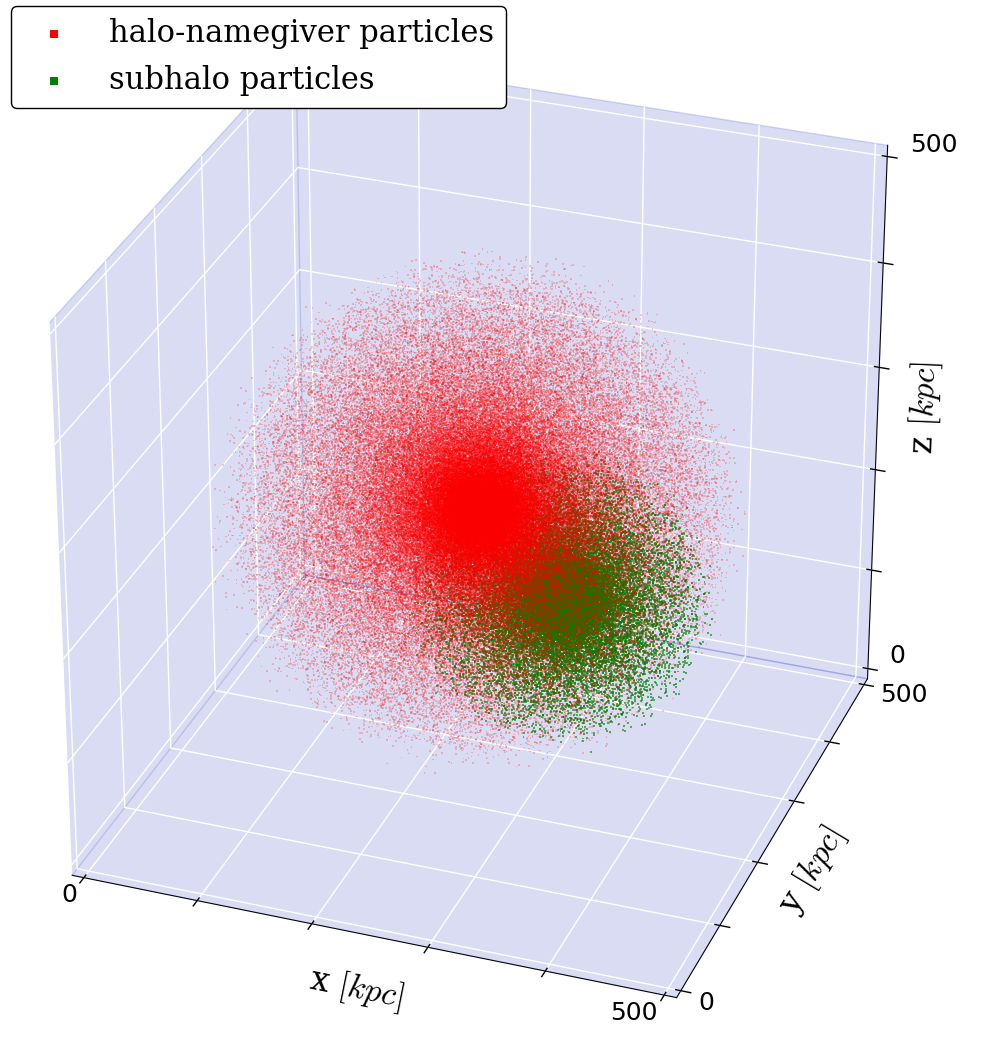
\includegraphics[width = .4\textwidth]{../report/images/dice-two/dice-two-original-plot.png}} \hspace*{-1em} 	& 
			{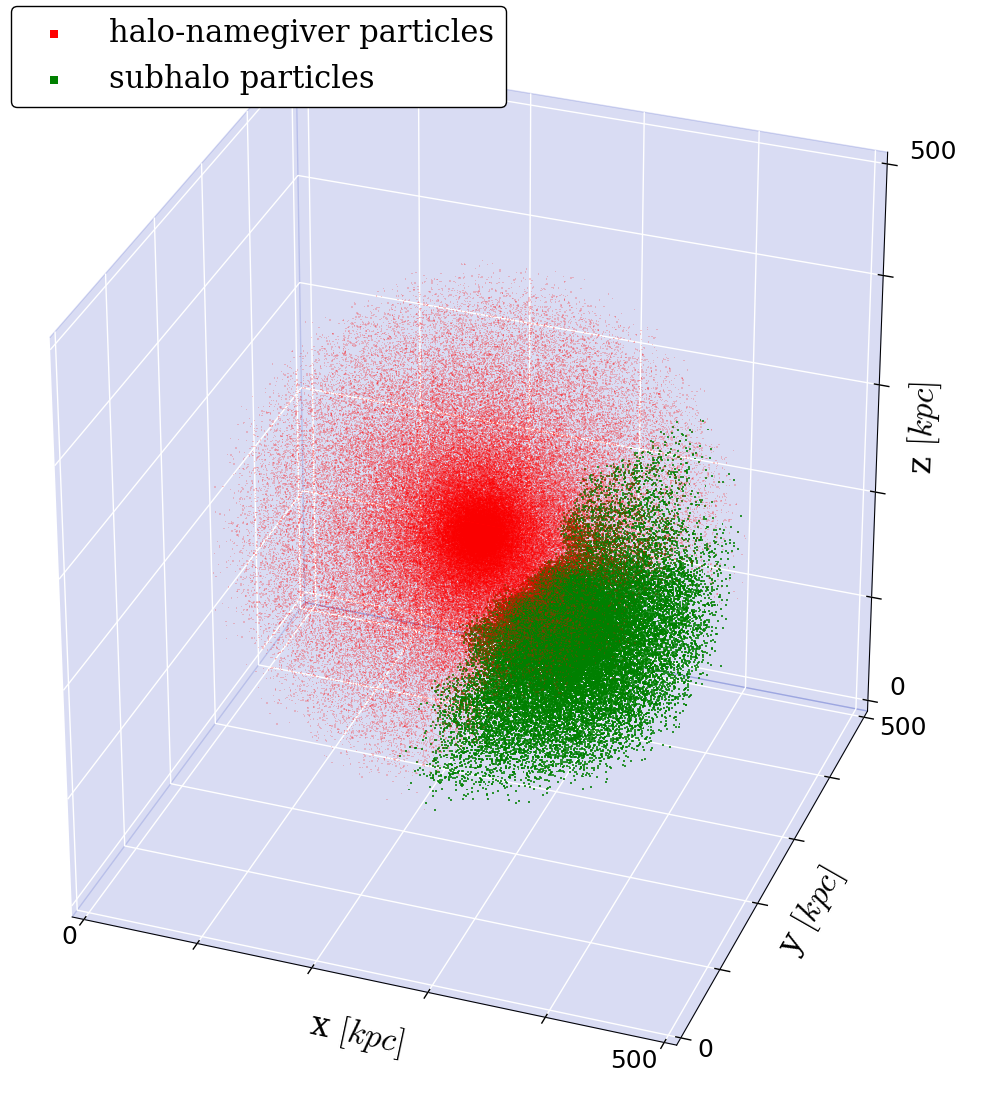
\includegraphics[width = .4\textwidth]{../report/images/dice-two/dice-two-plot-halo1451-phew.png}}
		\end{tabular}
	\end{center}

	The identified clump properties will be biased:
	\begin{itemize}
		\item Missing particles: Subhalo is cut off
		\item Alien particles: Subhalo in contaminated by host's particles
	\end{itemize}
\end{frame}



\begin{frame}
	\frametitle{Biased Clump Properties}
	
	It seems likely that the clump properties after particle unbinding should be closer to the known ones, particularly so if only exclusively bound particles are considered.\\[1em]
	
	$\Rightarrow$  recompute the clump properties after unbinding and use this updated information to go through the entire procedure again.
	
	Reiterate until the bulk velocity of each clump converges:
	\begin{equation*}
	\text{bulk velocity converged} \Leftrightarrow \left | \frac{v_{bulk,old} - v_{bulk,new}}{v_{bulk,old}} \right | < \varepsilon
	\end{equation*}
	where $\varepsilon$ is a user-defined convergence limit.
\end{frame}


\begin{frame}
	\frametitle{Results: Converging of the bulk velocity for the \dt-dataset}
	
The deviation $D_{orig} = \left | 	 \frac{v_{bulk} - v_{orig}}{v_{orig}}				\right |$  from the originally set bulk velocity to the computed bulk velocity for the subhalo of the \dt-dataset in dependence of the convergence limit $\varepsilon$:

	
	\begin{table}[!htb]
		\begin{centering}
			\begin{tabular}[t]{r | l | r | l }
				$\varepsilon$     &  \texttt{niter}  		&	$D_{orig}$	\\
				\hline
				0.5       &    	 		2    	&	0.2326  \\
				0.1       &   	       	4    	&	0.0419	\\
				0.01      &           	7    	&	0.0024	\\
				0.001     &            	8    	&	0.0014  \\       
				0.0001    &        		10    	&	0.0009 	\\
			\end{tabular}
		\end{centering}
	\end{table}
	
	The bulk velocity computation needed \texttt{niter} iterations to converge.
	
\end{frame}




\begin{frame}
	\frametitle{Results: \dt-dataset}
	
	\begin{tabular}{c c}
		\neigh\ 	& \iter \\[1.5em]
		%
		%	 
		{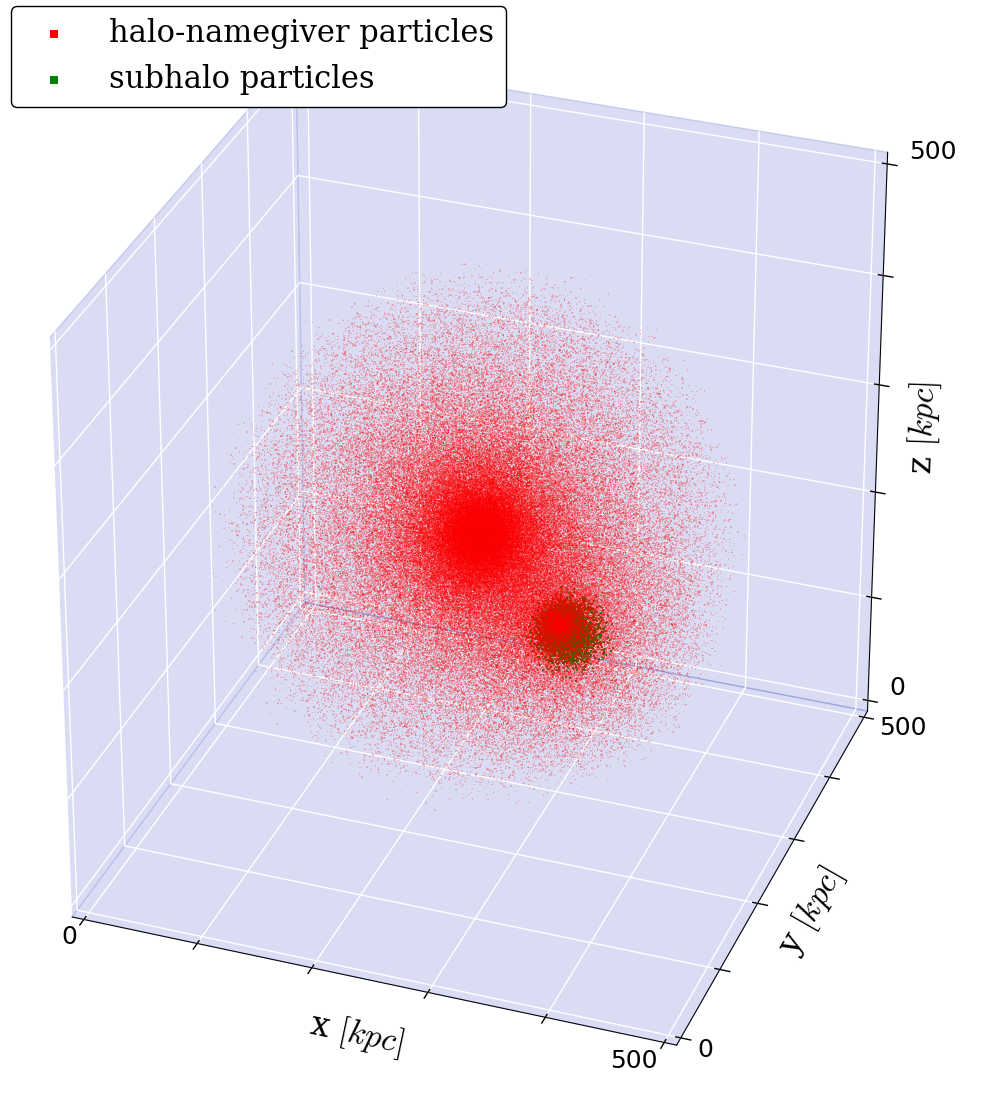
\includegraphics[width = .49\textwidth]{../report/images/dice-two/dice-two-plot-halo1451-saddle.png}} &
		{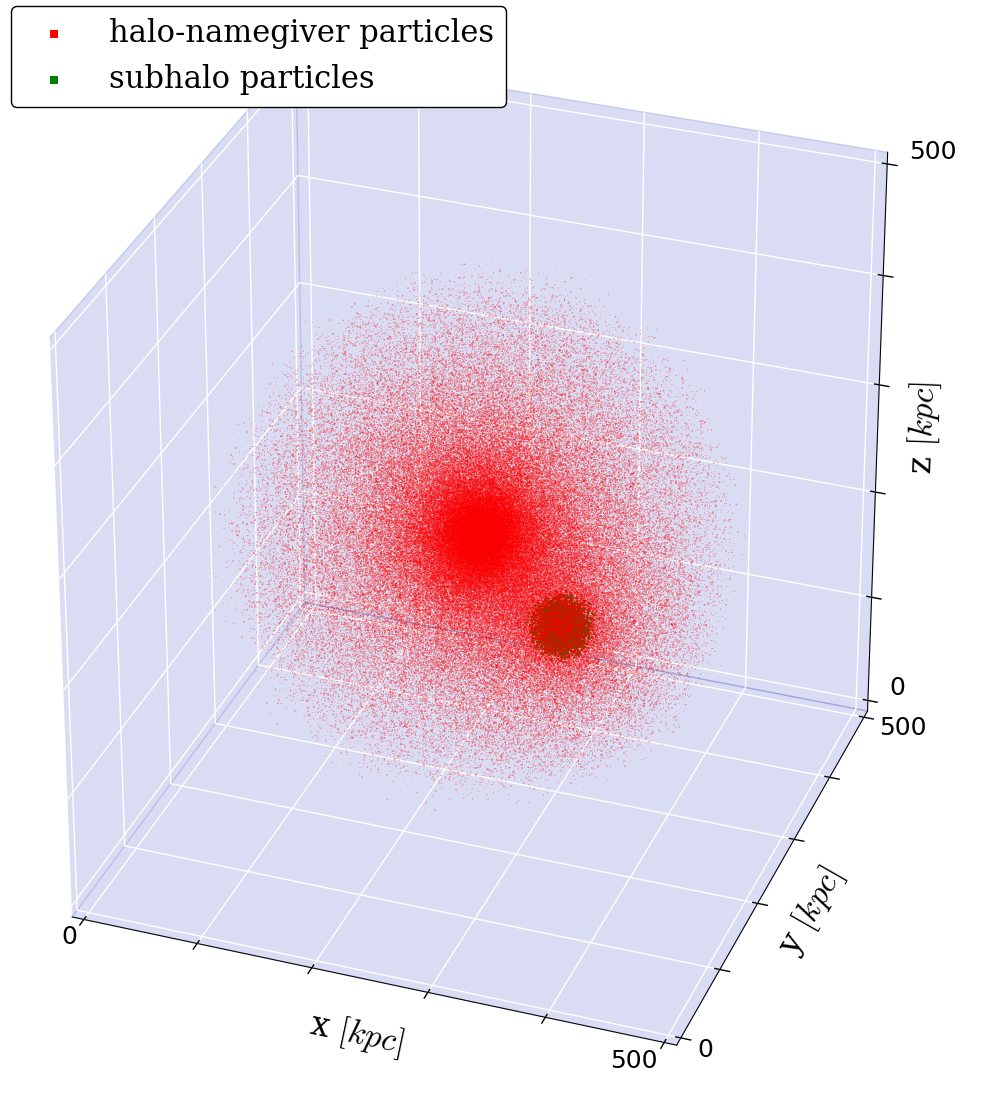
\includegraphics[width = .49\textwidth]{../report/images/dice-two/dice-two-plot-halo1451-iter.png}} \hspace*{-1em} 
	\end{tabular}
\end{frame}





\begin{frame}
	\frametitle{Results: \dt-dataset: halo-namegiver particles only}
	
	\begin{tabular}{c c}
		\neigh\ 	& \iter \\[1.5em]
		%
		%	 
		{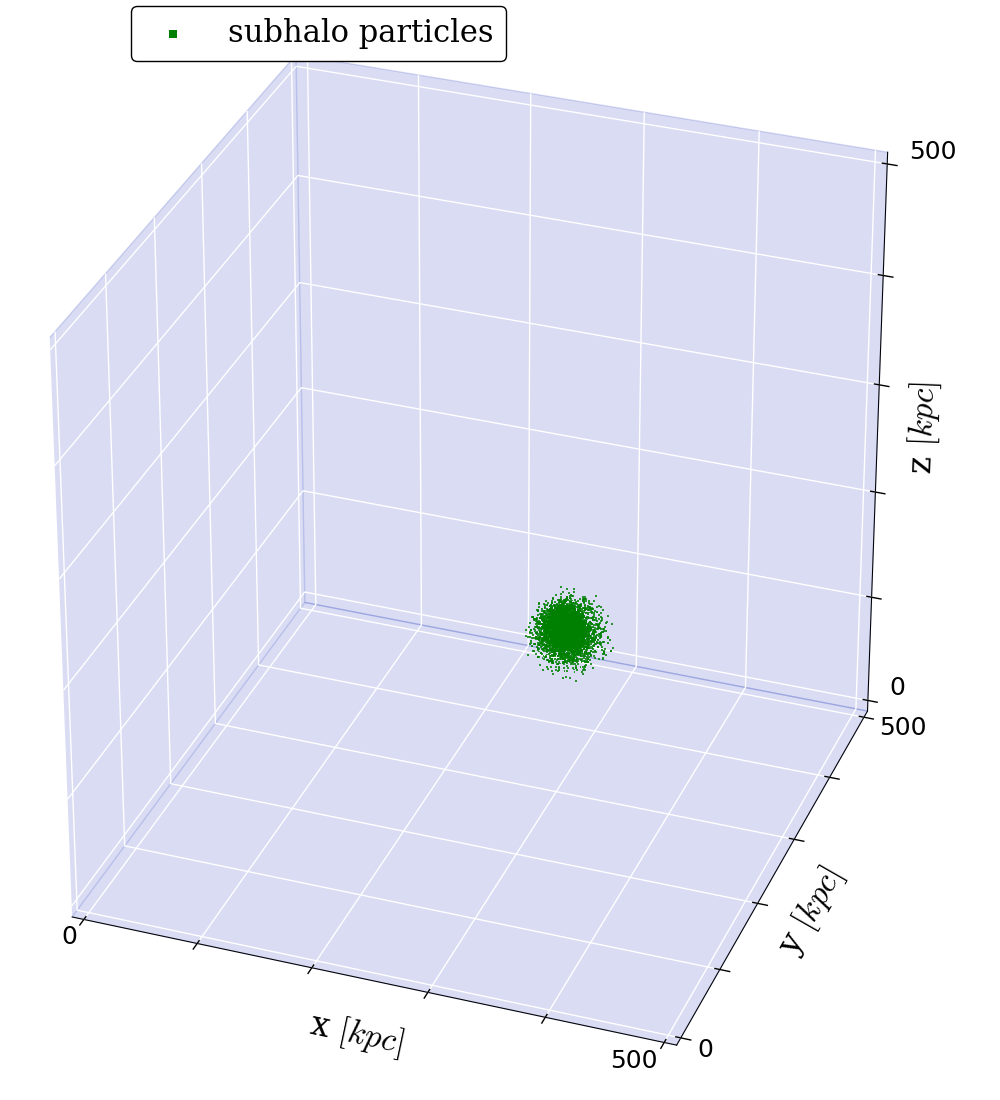
\includegraphics[width = .49\textwidth]{../report/images/dice-two/dice-two-plot-subhalo-saddle.png}}	&
		{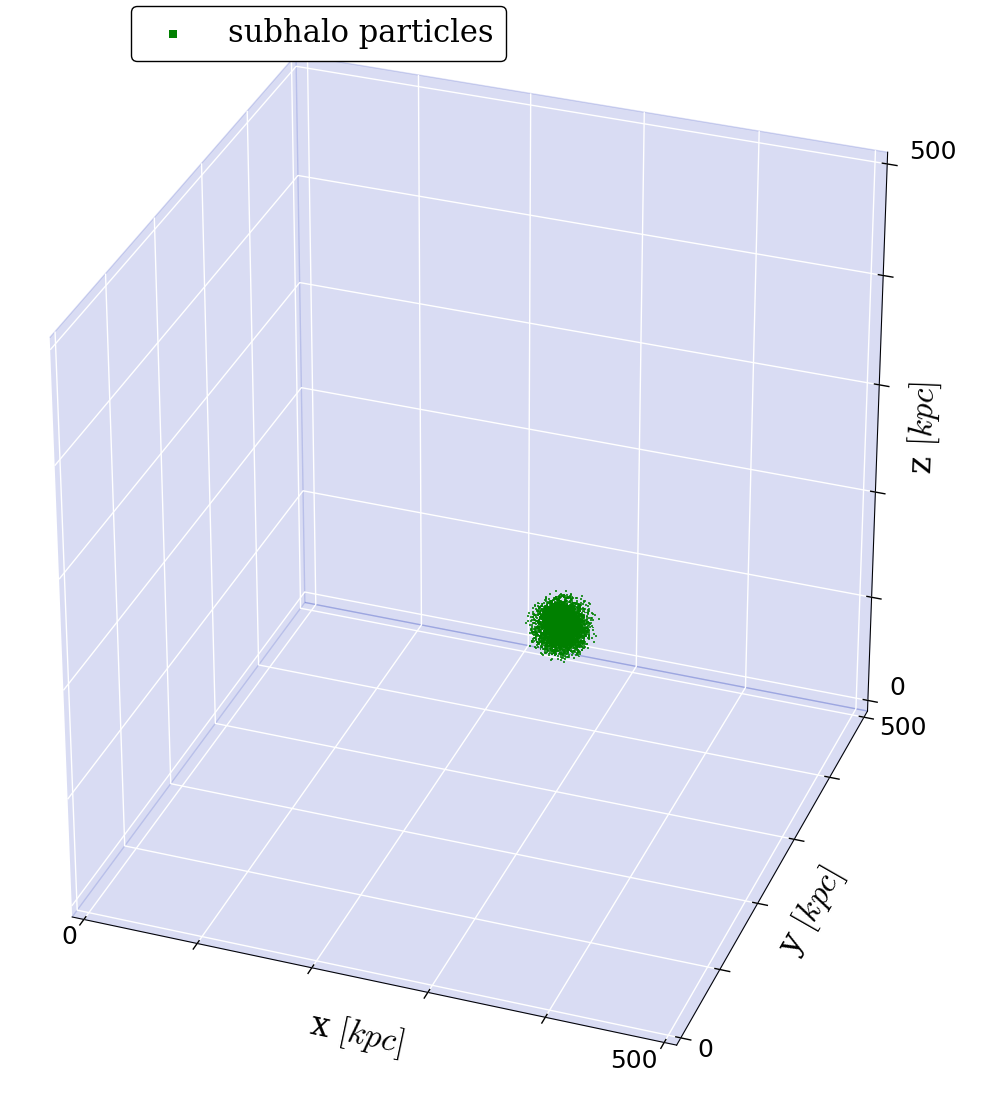
\includegraphics[width = .49\textwidth]{../report/images/dice-two/dice-two-plot-subhalo-iter.png}}  
	\end{tabular}
\end{frame}




%\begin{frame}
%	\frametitle{Results: \ds-dataset}
%	
%	\begin{tabular}{c c}
%		\neigh\ 	& \iter \\[1.5em]
%		%
%		%
%		
%		{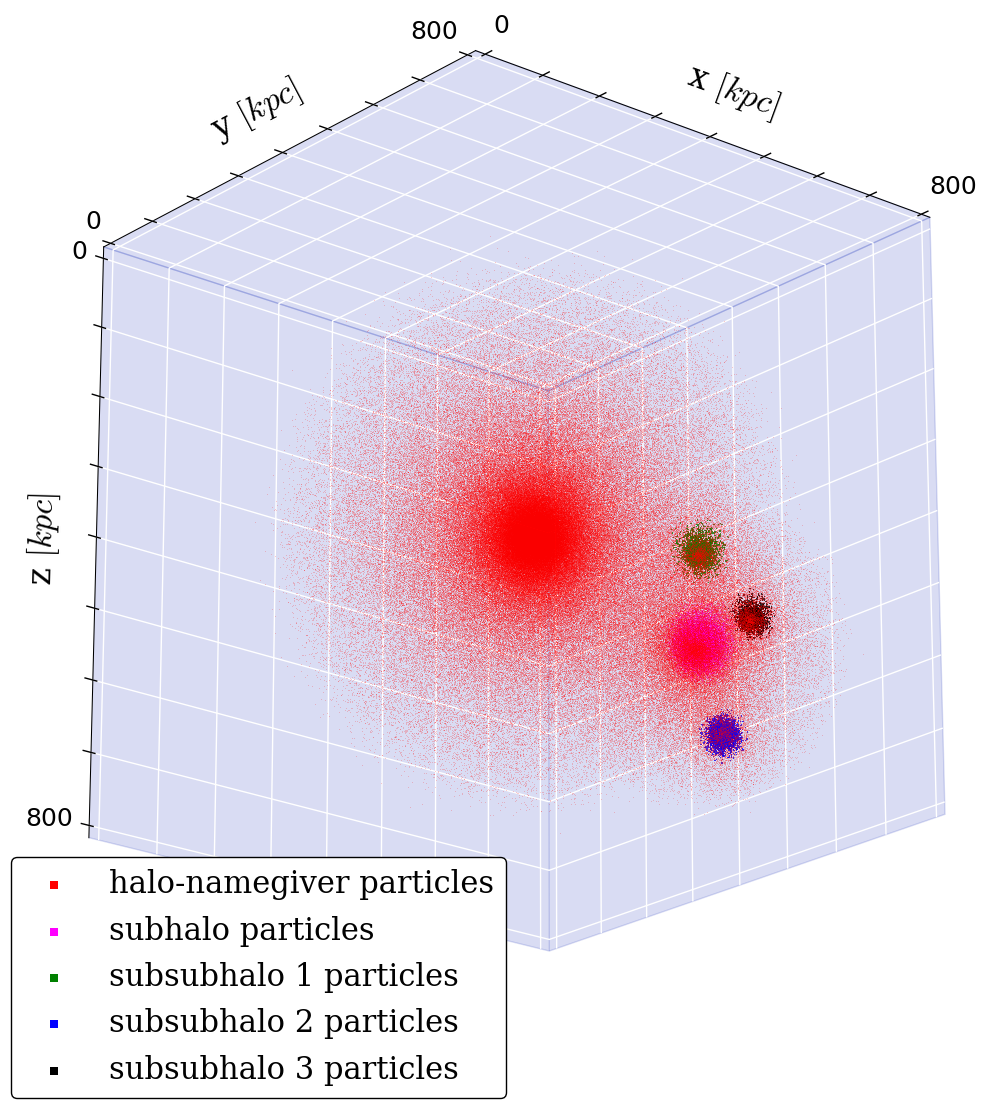
\includegraphics[width = .49\textwidth]{../report/images/dice-sub/dice-sub-plot-halo1-saddle.png}}	&		 
%		{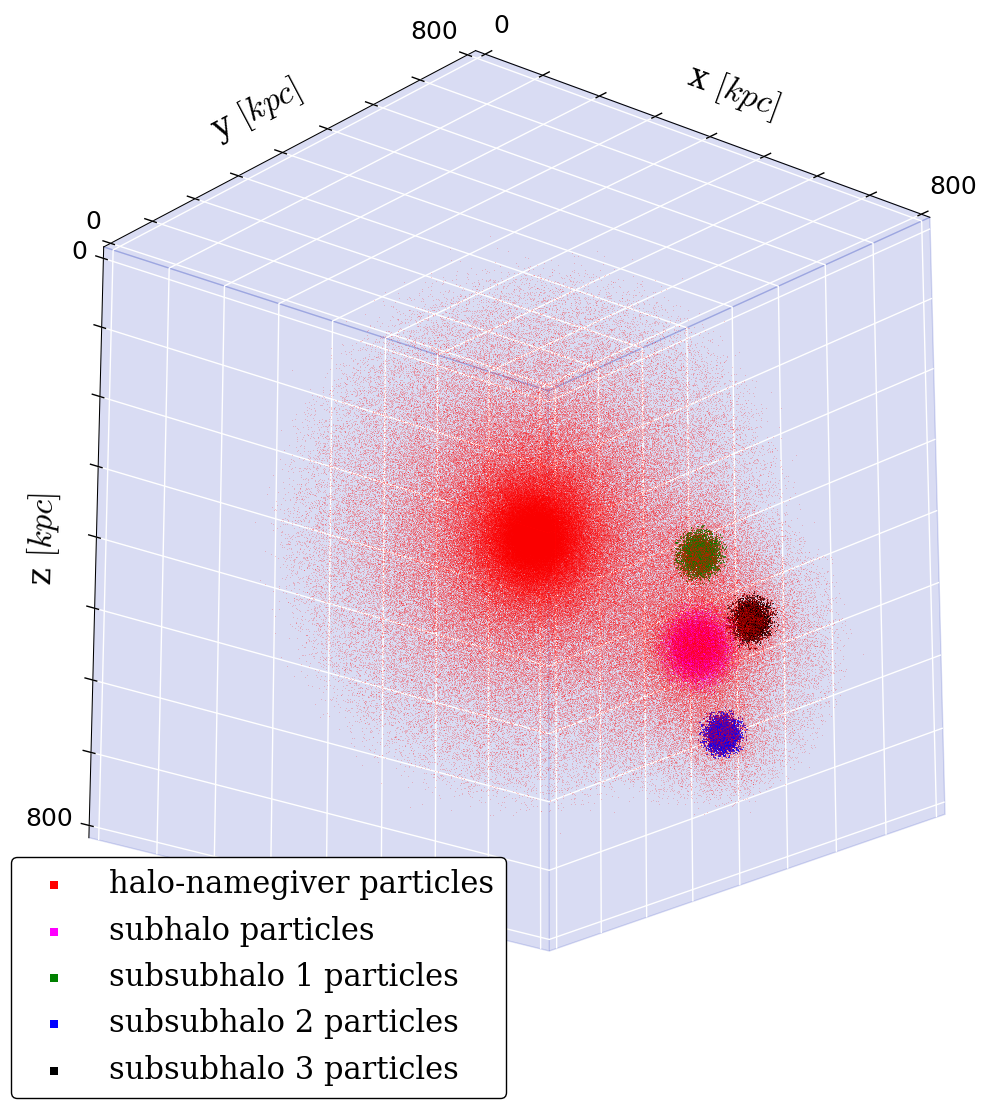
\includegraphics[width = .49\textwidth]{../report/images/dice-sub/dice-sub-plot-halo1-iter.png}} 	
%	\end{tabular}
%\end{frame}
%
%
%
%\begin{frame}
%	\frametitle{Results: \ds-dataset: halo-namegiver particles only}
%	
%	\begin{tabular}{c c}
%		\neigh\ 	& \iter \\[1.5em]
%		%
%		%	 
%		{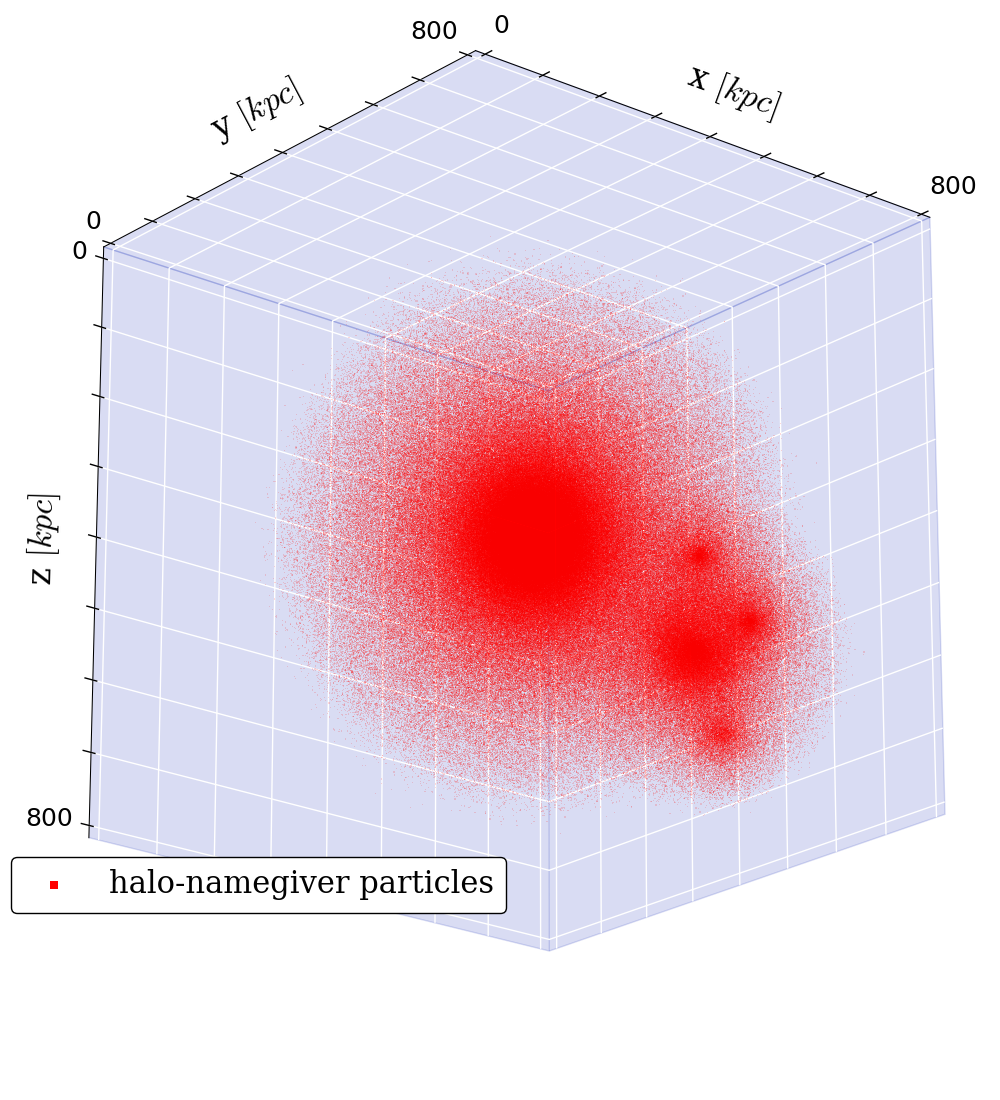
\includegraphics[width = .49\textwidth]{../report/images/dice-sub/dice-sub-halo-only-saddle.png}} \hspace*{-1em} 	& 
%		{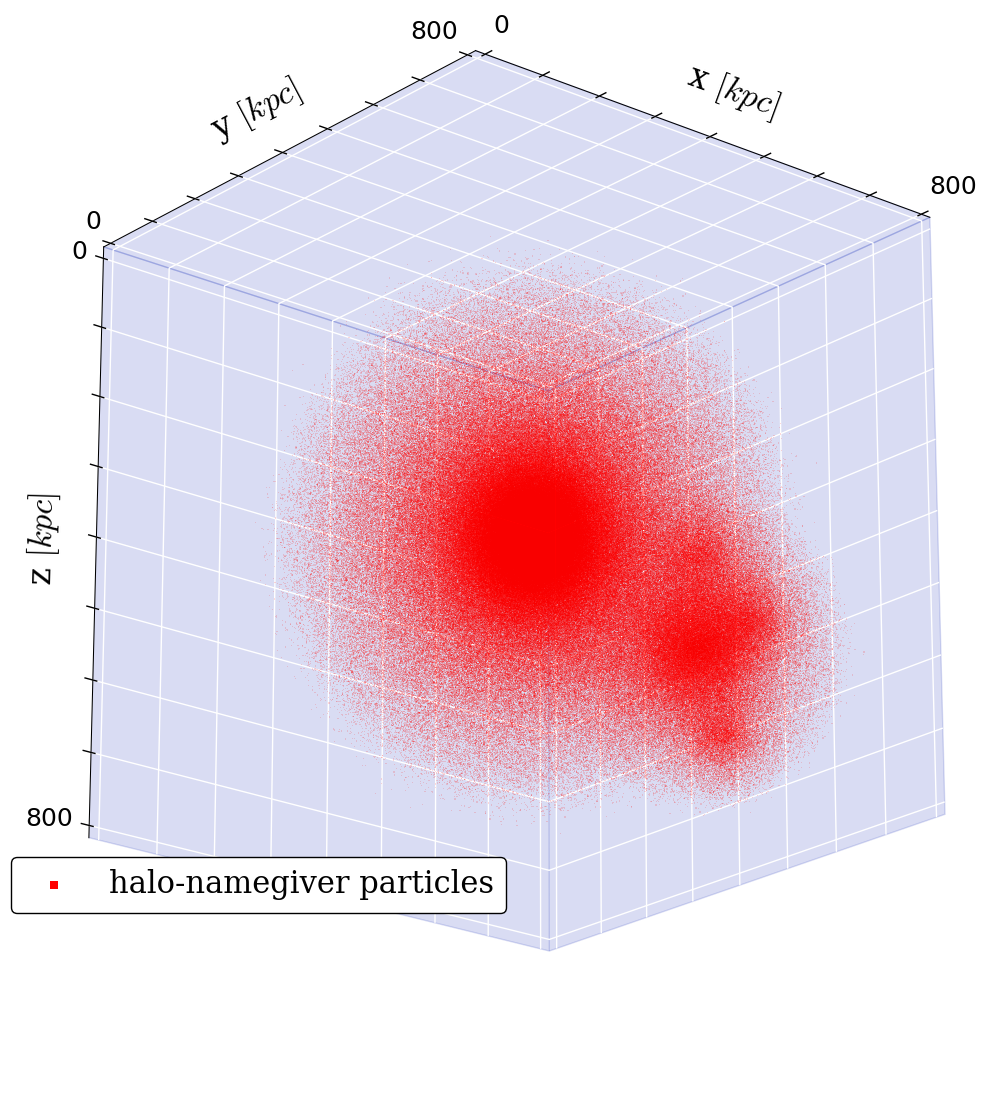
\includegraphics[width = .49\textwidth]{../report/images/dice-sub/dice-sub-halo-only-iter.png}}
%	\end{tabular}
%\end{frame}



\begin{frame}
	\frametitle{Results: \cosmo-dataset: halo-namegiver particles only}
	
	\begin{tabular}{c c}
		\neigh\ 	& \iter \\[1.5em]
		%
		%	 
		{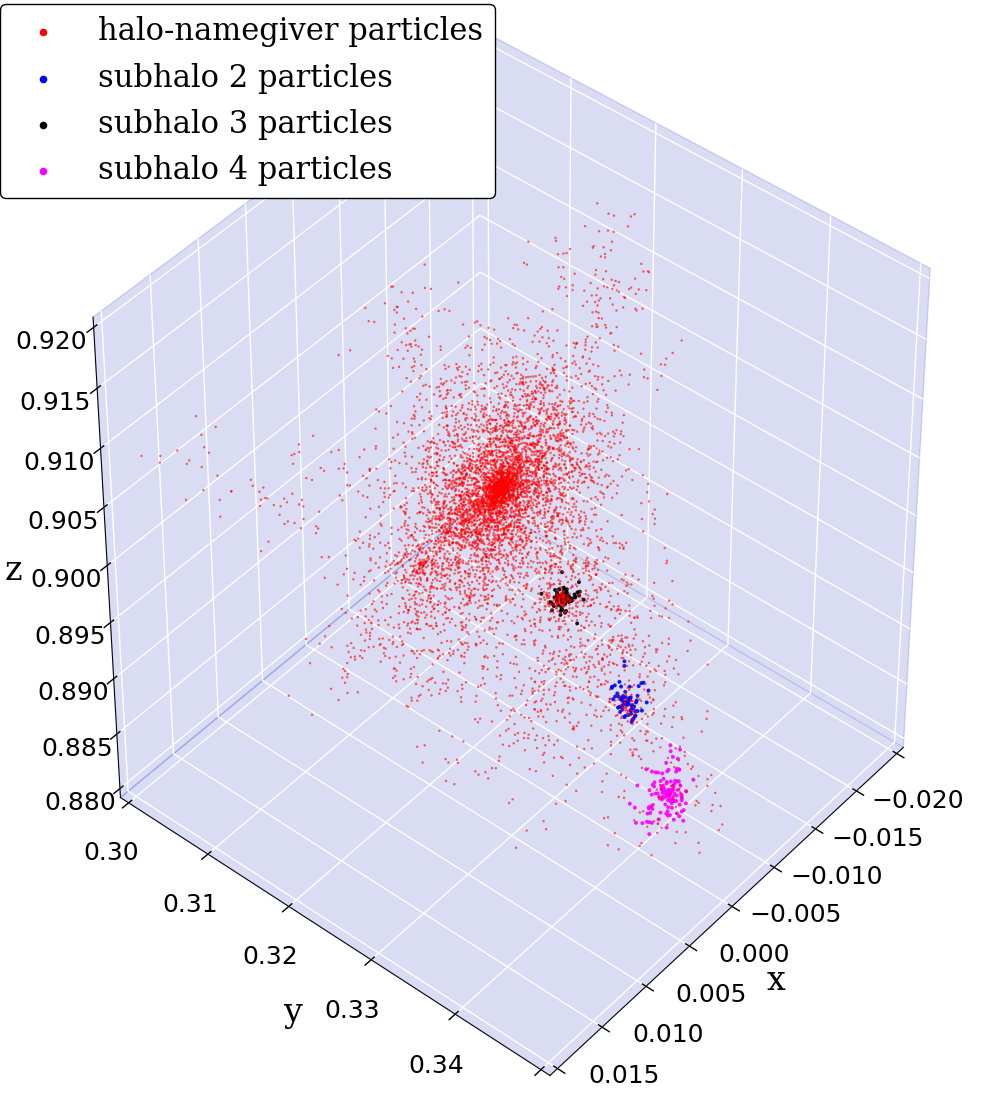
\includegraphics[width = .49\textwidth]{../report/images/cosmo/cos-halo-66858-saddle.png}}	& 
		{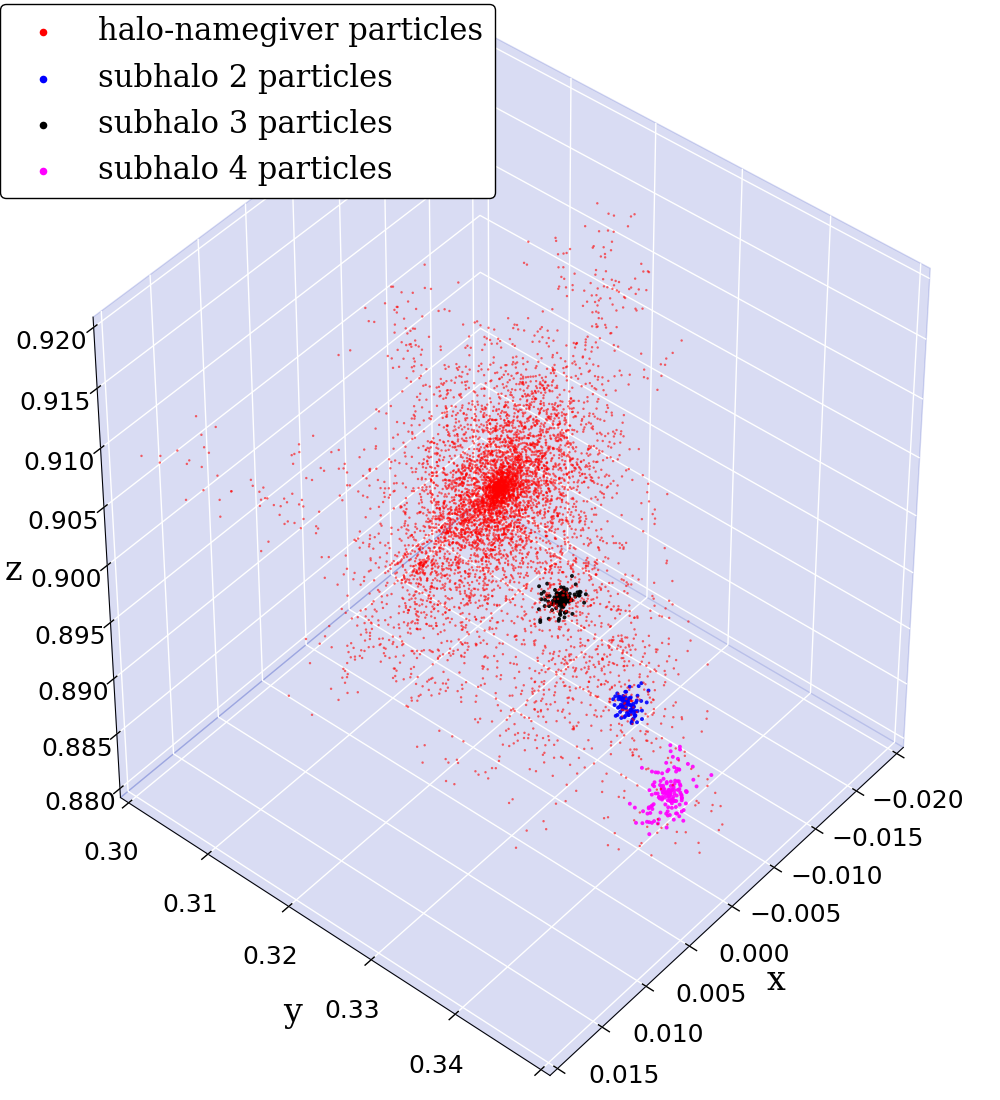
\includegraphics[width = .49\textwidth]{../report/images/cosmo/cos-halo-66858-iter.png}}
	\end{tabular}
\end{frame}



\begin{frame}
	\frametitle{Results: \cosmo-dataset: halo-namegiver particles only}
	
	\begin{tabular}{c c}
		\neigh\ 	& \iter \\[1.5em]
		%
		%	 
		{\includegraphics[width = .49\textwidth]{../report/images/cosmo/cos-halo-66858-halo-only-saddle.png}} \hspace*{-1em} 	& 
		{\includegraphics[width = .49\textwidth]{../report/images/cosmo/cos-halo-66858-halo-only-iter.png}}
	\end{tabular}
\end{frame}





\begin{frame}
	\frametitle{References}
	\renewcommand*{\bibfont}{\footnotesize}
	
	\printbibliography
\end{frame}

\begin{frame}
\end{frame}














\end{document}
